% Options for packages loaded elsewhere
\PassOptionsToPackage{unicode}{hyperref}
\PassOptionsToPackage{hyphens}{url}
%
\documentclass[
]{article}
\usepackage{amsmath,amssymb}
\usepackage{lmodern}
\usepackage{iftex}
\ifPDFTeX
  \usepackage[T1]{fontenc}
  \usepackage[utf8]{inputenc}
  \usepackage{textcomp} % provide euro and other symbols
\else % if luatex or xetex
  \usepackage{unicode-math}
  \defaultfontfeatures{Scale=MatchLowercase}
  \defaultfontfeatures[\rmfamily]{Ligatures=TeX,Scale=1}
\fi
% Use upquote if available, for straight quotes in verbatim environments
\IfFileExists{upquote.sty}{\usepackage{upquote}}{}
\IfFileExists{microtype.sty}{% use microtype if available
  \usepackage[]{microtype}
  \UseMicrotypeSet[protrusion]{basicmath} % disable protrusion for tt fonts
}{}
\makeatletter
\@ifundefined{KOMAClassName}{% if non-KOMA class
  \IfFileExists{parskip.sty}{%
    \usepackage{parskip}
  }{% else
    \setlength{\parindent}{0pt}
    \setlength{\parskip}{6pt plus 2pt minus 1pt}}
}{% if KOMA class
  \KOMAoptions{parskip=half}}
\makeatother
\usepackage{xcolor}
\usepackage[margin=1in]{geometry}
\usepackage{graphicx}
\makeatletter
\def\maxwidth{\ifdim\Gin@nat@width>\linewidth\linewidth\else\Gin@nat@width\fi}
\def\maxheight{\ifdim\Gin@nat@height>\textheight\textheight\else\Gin@nat@height\fi}
\makeatother
% Scale images if necessary, so that they will not overflow the page
% margins by default, and it is still possible to overwrite the defaults
% using explicit options in \includegraphics[width, height, ...]{}
\setkeys{Gin}{width=\maxwidth,height=\maxheight,keepaspectratio}
% Set default figure placement to htbp
\makeatletter
\def\fps@figure{htbp}
\makeatother
\setlength{\emergencystretch}{3em} % prevent overfull lines
\providecommand{\tightlist}{%
  \setlength{\itemsep}{0pt}\setlength{\parskip}{0pt}}
\setcounter{secnumdepth}{-\maxdimen} % remove section numbering
\usepackage{booktabs}
\usepackage{longtable}
\usepackage{array}
\usepackage{multirow}
\usepackage{wrapfig}
\usepackage{float}
\usepackage{colortbl}
\usepackage{pdflscape}
\usepackage{tabu}
\usepackage{threeparttable}
\usepackage{threeparttablex}
\usepackage[normalem]{ulem}
\usepackage{makecell}
\usepackage{xcolor}
\ifLuaTeX
  \usepackage{selnolig}  % disable illegal ligatures
\fi
\IfFileExists{bookmark.sty}{\usepackage{bookmark}}{\usepackage{hyperref}}
\IfFileExists{xurl.sty}{\usepackage{xurl}}{} % add URL line breaks if available
\urlstyle{same} % disable monospaced font for URLs
\hypersetup{
  pdftitle={Nhanes 2021 Blood Pressure-Based Mortality Risk - Appendix A},
  pdfauthor={Rscripts by Hamish Patten, DW Bester and David Steinsaltz},
  hidelinks,
  pdfcreator={LaTeX via pandoc}}

\title{Nhanes 2021 Blood Pressure-Based Mortality Risk - Appendix A}
\author{Rscripts by Hamish Patten, DW Bester and David Steinsaltz}
\date{21/07/2022}

\begin{document}
\maketitle

{
\setcounter{tocdepth}{3}
\tableofcontents
}
\hypertarget{appendix-a---further-detail-on-modelling-and-results}{%
\section{Appendix A - Further Detail on Modelling and
Results}\label{appendix-a---further-detail-on-modelling-and-results}}

This appendix aims to add more detail about the numerical modelling than
was provided in the article. This is to ensure that the research methods
are transparent and entirely reproducible. The numerical modelling
presented in this paper was performed using R combined with Rstan. More
detail will be provided here about the model, about the specific
methodology used to parameterize the model, and more results are
provided that were not included in the main bulk of the article.

\hypertarget{model}{%
\subsection{Model}\label{model}}

The model used in this research is built from the theory of joint
modelling of longitudinal and time-to-event data. This will be described
in detail later on in this section, however, in brief, this allows the
simultaneous modelling of both longitudinal observation data (in this
article, this is blood pressure measurements) and also the time-to-event
outcome. In this research the event of interest is either death from any
cause, or death from specifically cardiovascular or cerebrovascular
disease (CVD). In the latter case death from a different cause is
treated as a noninformative censoring event.

\hypertarget{survival-analysis-time-to-event}{%
\subsubsection{Survival Analysis
(Time-to-Event)}\label{survival-analysis-time-to-event}}

The basic survival model is a Gompertz hazard rate with proportional
hazards influences of the blood pressure covariates. The Gompertz
equation \begin{equation}\label{gompertz}
h_0(t)=B\exp{\left(\theta(x+T)\right)},
\end{equation} describes the baseline hazard of the population to a
particular risk, which, for this article, investigates CVD mortality
specifically, as well as studying mortality risk in general.
\(x\in\mathbb{N^N}\) is the age of the individual at the initial
interview time, for \(N\) the number of individuals, and
\(T\in\mathbb{R}^{+,N}\) the time since the individual entered the
survey. Note that both \(B\) and \(\theta\) have 6 different values,
depending on the sex reported at the initial interview -- female or male
--- or the race --- black, white or `other'. Note that `other' in the
race category is a combination of all non-black or non-white racial
identities, such as Hispanic populations. The log-linear proportional
hazards model links the covariates of the model (mean systolic blood
pressure, variance in the diastolic blood pressure, etc) to the survival
outcome of the individual via the equation
\begin{equation}\label{prophaz}
h(t)=h_0(t)\exp{\left(\boldsymbol{\beta}\cdot(\boldsymbol{X}-\hat{\boldsymbol{X}})\right)},
\end{equation} where \(\boldsymbol{X}\in\mathbb{R}^{+,N\times d}\) is a
vector of summary statistics of the blood pressure measurements of
individual covariates in our model,
\(\hat{\boldsymbol{X}}\in\mathbb{R}^{+,d}\) is the centering of the
covariates such that the equation
\(\sum_i^N \exp{(\boldsymbol{\beta}\cdot(\boldsymbol{X}-\hat{\boldsymbol{X}}))}=0\)
is approximately satisfied (more on this later), and
\(\boldsymbol{\beta}\in\mathbb{R}^d\) implies the strength of the
influence of the covariate on the mortality risk. The majority of
mortality events are censored --- not yet known at the time of data
collection --- the censoring indicator being notated as
\(\delta\in \{0,1\}\). When CVD mortality is the event being analysed,
deaths due to other causes are treated as noninformative censoring
events. In this study, we explored the following covariates:

\begin{tabular}{lll}
\toprule
Variable Name & Support & Description\\
\midrule
$FRS-1998$ & $R^N$ & 1998 version of the FRS score\\
$FRS-ATP$ & $R^N$ & ATP version of the FRS score\\
$M_S$ & $R^{+,N}$ & Mean systolic blood pressure\\
$M_D$ & $R^{+,N}$ & Mean diastolic blood pressure\\
$\Delta_S$ & $R^{+,N}$ & Difference between Home and Clinic mean systolic blood pressure\\
\addlinespace
$\Delta_D$ & $R^{+,N}$ & Difference between Home and Clinic mean diastolic blood pressure\\
$\sigma_{\{S,H\}}$ & $R^{+,N}$ & Standard deviation of the systolic blood pressure taken at home\\
$\sigma_{\{D,H\}}$ & $R^{+,N}$ & Standard deviation of the diastolic blood pressure taken at home\\
$\sigma_{\{S,C\}}$ & $R^{+,N}$ & Standard deviation of the systolic blood pressure taken at the clinic\\
$\sigma_{\{D,C\}}$ & $R^{+,N}$ & Standard deviation of the diastolic blood pressure taken at the clinic\\
\addlinespace
$\tau_{\{S,H\}}$ & $R^{+,N}$ & Precision of the systolic blood pressure taken at home\\
$\tau_{\{D,H\}}$ & $R^{+,N}$ & Precision of the diastolic blood pressure taken at home\\
$\tau_{\{S,C\}}$ & $R^{+,N}$ & Precision of the systolic blood pressure taken at the clinic\\
$\tau_{\{D,C\}}$ & $R^{+,N}$ & Precision of the diastolic blood pressure taken at the clinic\\
\bottomrule
\end{tabular}

Please note that the last four elements of this list, the precision
values, were only carried out to ensure model consistency with the use
of standard deviation instead. Note as well that the \(\Delta\)
covariates, representing the medium-term variability, enter into the log
relative risk sum as an \textbf{absolute value}.

For the parametrization of this model, we assume that the Gompertz
parameters and the parameters in the linear predictor term are
distributed as follows: \begin{equation}\label{priorsS}
\begin{aligned}
  \boldsymbol{B}\sim\mathbb{C}(\mu_B,\sigma_B),\\
  \boldsymbol{\theta}\sim\mathfrak{N}(\mu_\theta,\sigma_\theta),\\
  \boldsymbol{\beta}\sim \mathfrak{N}(\mu_\beta,\sigma_\beta),
\end{aligned}
\end{equation} noting that \(\mathbb{C}(\mu,\sigma)\) is the Cauchy
distribution.

The likelihood for this Gompertz proportional hazards model, over all
individuals in the census, is as follows:
\begin{equation}\label{likesurv}
L_S(\boldsymbol{v},\boldsymbol{\delta})=\prod_i^N f(v_i,\delta_i|B_i,\theta_i,\beta_i,\boldsymbol{X},\hat{\boldsymbol{X}})=\prod_i^N h(v_i|B_i,\theta_i,\beta_i,\boldsymbol{X},\hat{\boldsymbol{X}})^{\delta_i} \exp{\left( -\sum_i^N H(v_i|B_i,\theta_i,\beta_i,\boldsymbol{X},\hat{\boldsymbol{X}}) \right)},
\end{equation} with \(H(v)=\int_0^v h(w)dw\) the cumulative hazard.

\hypertarget{longitudinal-modelling}{%
\subsubsection{Longitudinal Modelling}\label{longitudinal-modelling}}

The mortality hazard rates are assumed to be influenced by
individual-level blood pressure means and variability characteristics.
These characteristics are not directly observed, but are inferred from
their influence on the individual blood pressure measurements, which
have been observed. Let \(Y_i(t_j)\) be the observed blood pressure for
patient \(i\) at time \(t_j\), for the individual \(i\in 1,2,...,N\) and
the number of blood pressure measurements per individual
\(j\in 1,2,...,k\). Due to the fact that the blood pressure measurement
data was taken at both the home and clinic (written using subscripts H
and C, respectively), with approximately 6 months between these two
measurements, we model the blood pressure using the following model,
assuming the diastolic \(Y_{i}^D\) and systolic \(Y_{i}^S\) blood
pressure to be Gaussian-distributed: \begin{equation}\label{bp}
\begin{aligned}
  (Y_{i}^D)_{H} \sim \mathfrak{N}(M_i^D+\Delta_i^D,(\sigma_i^D)_H),\\
  (Y_{i}^D)_{C} \sim \mathfrak{N}(M_i^D-\Delta_i^D,(\sigma_i^D)_C),\\
  (Y_{i}^S)_{H} \sim \mathfrak{N}(M_i^S+\Delta_i^S,(\sigma_i^S)_H),\\
  (Y_{i}^S)_{C} \sim \mathfrak{N}(M_i^S-\Delta_i^S,(\sigma_i^S)_C),
\end{aligned}
\end{equation} where superscripts \(D\) and \(S\) refer to diastolic and
systolic blood pressure, respectively.

The blood pressure characteristics --- the individual-level parameters
--- are themselves distributed according to a hierarchical model,
determined by population-level parameters (also called
``hyperparameters'\,'): \begin{equation}\label{priorsL}
\begin{aligned}
  M_i^{\{D,S\}}\sim \mathfrak{N}(\mu_M^{\{D,S\}},\sigma_M^{\{D,S\}}),\\
  \Delta_i^{\{D,S\}}\sim \mathfrak{N}(\mu_D^{\{D,S\}},\sigma_D^{\{D,S\}}),\\
  \sigma_{i,C}^{\{D,S\}}\sim \Gamma(r_C^{\{D,S\}},\lambda_C^{\{D,S\}}),\\
  \sigma_{i,H}^{\{D,S\}}\sim \Gamma(r_H^{\{D,S\}},\lambda_H^{\{D,S\}}).
\end{aligned}
\end{equation} The longitudinal outcome modelling therefore aims to
infer these hyperparameters \begin{equation}
  \Theta=\left\{\mu_M^{\{D,S\}},\mu_D^{\{D,S\}},\sigma_M^{\{D,S\}},\sigma_D^{\{D,S\}},r_C^{\{D,S\}},\lambda_C^{\{D,S\}},r_H^{\{D,S\}},\lambda_H^{\{D,S\}}\right\},
\end{equation} and to use the implied uncertainty about the
individual-level parameters to inform the inference about the survival
parameters. The likelihood for the longitudinal measurements is
therefore (combining the systolic and diastolic into a single parameter
for simplicity): \begin{equation}\label{likelong}
  L_L(\Theta|Y)=\prod_{i=1}^N\left(\prod_{j=1}^{k}f(y_{ij}|M_i,\Delta_i,\sigma_i)\right)f(M_i|\mu_M,\sigma_M)f(\Delta_i|\mu_D,\sigma_D)f(\tau_{i,C}|r_C,\lambda_C)f(\tau_{i,H}|r_H,\lambda_H)
\end{equation}

\hypertarget{combined-hierarchical-model}{%
\subsubsection{Combined Hierarchical
Model}\label{combined-hierarchical-model}}

Combining the longitudinal outcome and time-to-event partial
likelihoods, and for a given parameter space value of
\(\Omega=\{\beta,B,\theta\}\cup \Theta\), the joint likelihood is
\begin{equation}
\begin{split}
  L(\Omega|Y)=\prod_{i=1}^N\left(\prod_{j=1}^{k}f(y_{ij}|M_i,\Delta_i,\sigma_i)\right)f&(v_i,\delta_i|B_i,\theta_i,\beta_i,\boldsymbol{X},\hat{\boldsymbol{X}})f(M_i|\mu_M,\sigma_M)\\
  &f(\Delta_i|\mu_D,\sigma_D)f(\tau_{i,C}|r_C,\lambda_C)f(\tau_{i,H}|r_H,\lambda_H).
  \end{split}
\end{equation} One approach to estimating the complete set of
hyperparameters \begin{equation}
  \Omega_H=\{\mu_B,\sigma_B,\mu_\theta,\sigma_\theta,\mu_\beta,\sigma_\beta,\mu_M^{\{D,S\}},\sigma_M^{\{D,S\}},\mu_D^{\{D,S\}},\sigma_D^{\{D,S\}},r_C^{\{D,S\}},\lambda_C^{\{D,S\}},r_H^{\{D,S\}},\lambda_H^{\{D,S\}}\}
\end{equation} is to impose a higher-level prior distribution, and use
the machinery of Bayesian inference to produce posteriors for
everything. This approach runs into computational difficulties, which
have led us to a two-stage ``empirical Bayes'\,' approach, where the
hyperparameters for the longitudinal model are first fixed by a
maximum-likelihood calculation, after which the remaining
hyperparameters and individual-level parameters can be estimated with
Bayesian machinery. For the time-to-event parameters we choose flat
hyperpriors, selecting the hyperparameters
\(\mu_B=\mu_\theta=\mu_\beta=0\), \(\sigma_B=\sigma_\theta=2\), and
\(\sigma_\beta=100\).

\hypertarget{the-modelling-variants}{%
\subsubsection{The modelling variants}\label{the-modelling-variants}}

In this article, we researched into 16 variants of the model-fitting
problem, but focussed mainly on 8 of them. The 8 main models use the
standard deviation, \(\sigma\), as the measure of the influence of
blood-pressure variability on mortality. We also produced the same 8
models but using precision, \(\tau=1/\sigma^2\), as the measure of the
influence of blood-pressure variability on mortality. However, this was
only to ensure that there were no differences between the use of one
over the other. Throughout the remainder of this appendix, we refer to
the 8 main models using the following run numbers:

\begin{enumerate}
\item All participants (15,295), using mean systolic and diastolic blood pressure (not FRS) in the linear predictor term, with the outcome data as death specifically from CVD.
\item All participants (15,295), using mean systolic and diastolic blood pressure (not FRS) in the linear predictor term, with the outcome data as all-causes of death.
\item Only participants that had data from which FRS values could be computed (N=9,418) --- the ``FRS population'' but using mean systolic and diastolic blood pressure (not FRS) in the linear predictor term, with the outcome data as death specifically from CVD.
\item FRS population, but using mean systolic and diastolic blood pressure (not FRS) in the linear predictor term, with the outcome data as all-causes of death.
\item FRS population, and using the FRS ATP-III value in the linear predictor term, with the outcome data as death specifically from CVD.
\item FRS population, and using the FRS ATP-III value in the linear predictor term, with the outcome data as all-causes of death.
\item FRS population, and using the FRS 1998-version value in the linear predictor term, with the outcome data as death specifically from CVD.
\item FRS population, and using the FRS 1998-version value in the linear predictor term, with the outcome data as all-causes of death.
\label{tab:runnums}
\end{enumerate}

We also include Directed Acyclical Graph (DAG) sketches to help
visualize the different models, as shown in figures \ref{fig:DAGmean}
and \ref{fig:DAGFRS}. In order to read the DAGs, note that each square
background layer that appears as a stack of layers represents different
measured outcomes that were made in the first wave of the survey. The
outcome variables measured are represented by a square-shaped text box,
and a parameter of the model is represented by a circular-shaped text
box. If either a square or circular text box is placed on top of a
stacked rectangular layer, it means that multiple values of that
variable (as many as there are layers to the stack) are either measured
(for outcome variables) or simulated (for parameters of the model).
Please note that the number of layers in the stack is written in the
text box that does not contain a frame which is intentionally displayed
on top of the stacked layer that it represents. For example,
\(i=1,...,N\). Finally, the direction of the arrows implies causality
assumed in the model.

\begin{figure}
\hypertarget{fig:DAGmean}{%
\centering
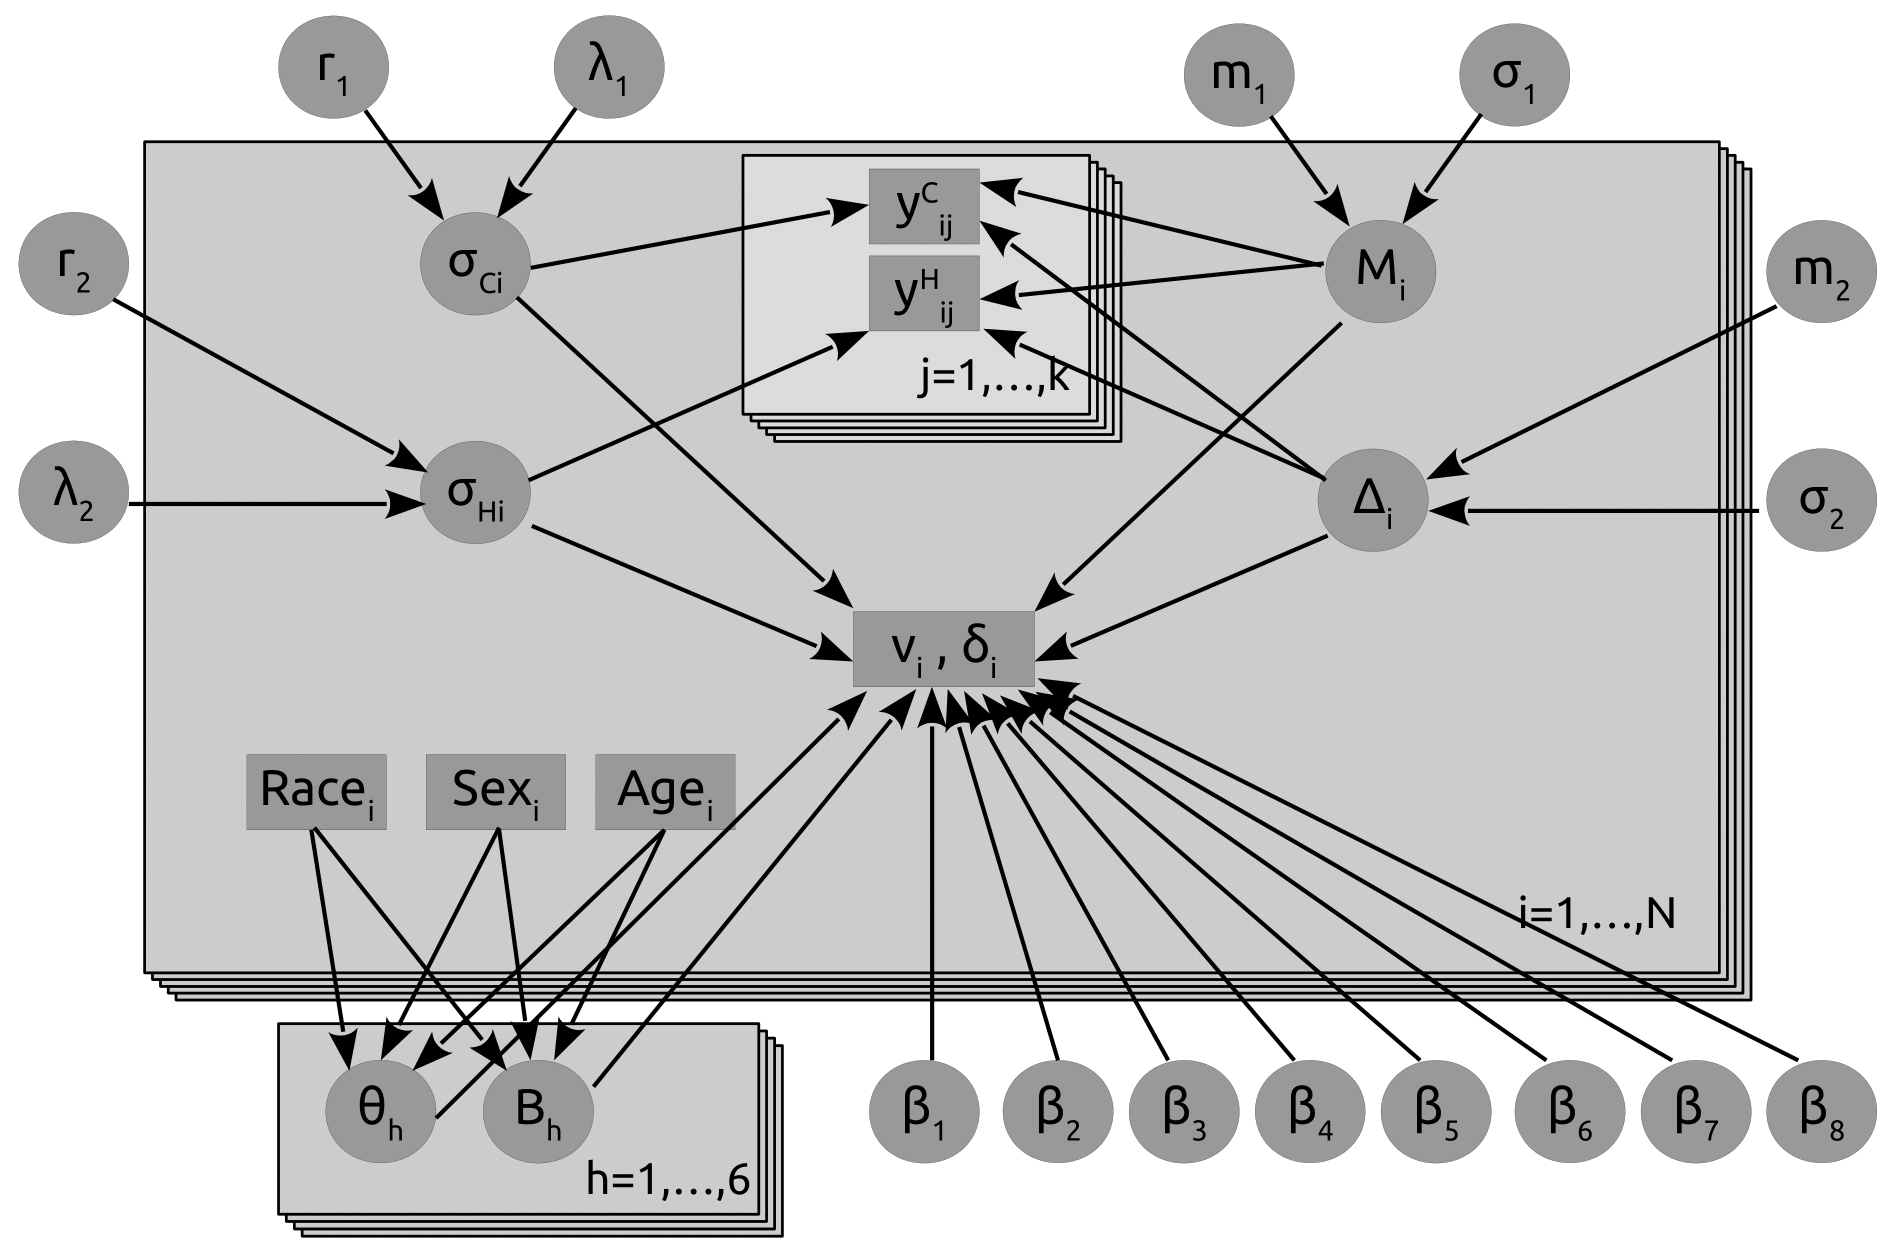
\includegraphics{./DAG_Mean.png}
\caption{An illustration of the DAG of the mean blood pressure-based
model presented in this article.}\label{fig:DAGmean}
}
\end{figure}

\begin{figure}
\hypertarget{fig:DAGFRS}{%
\centering
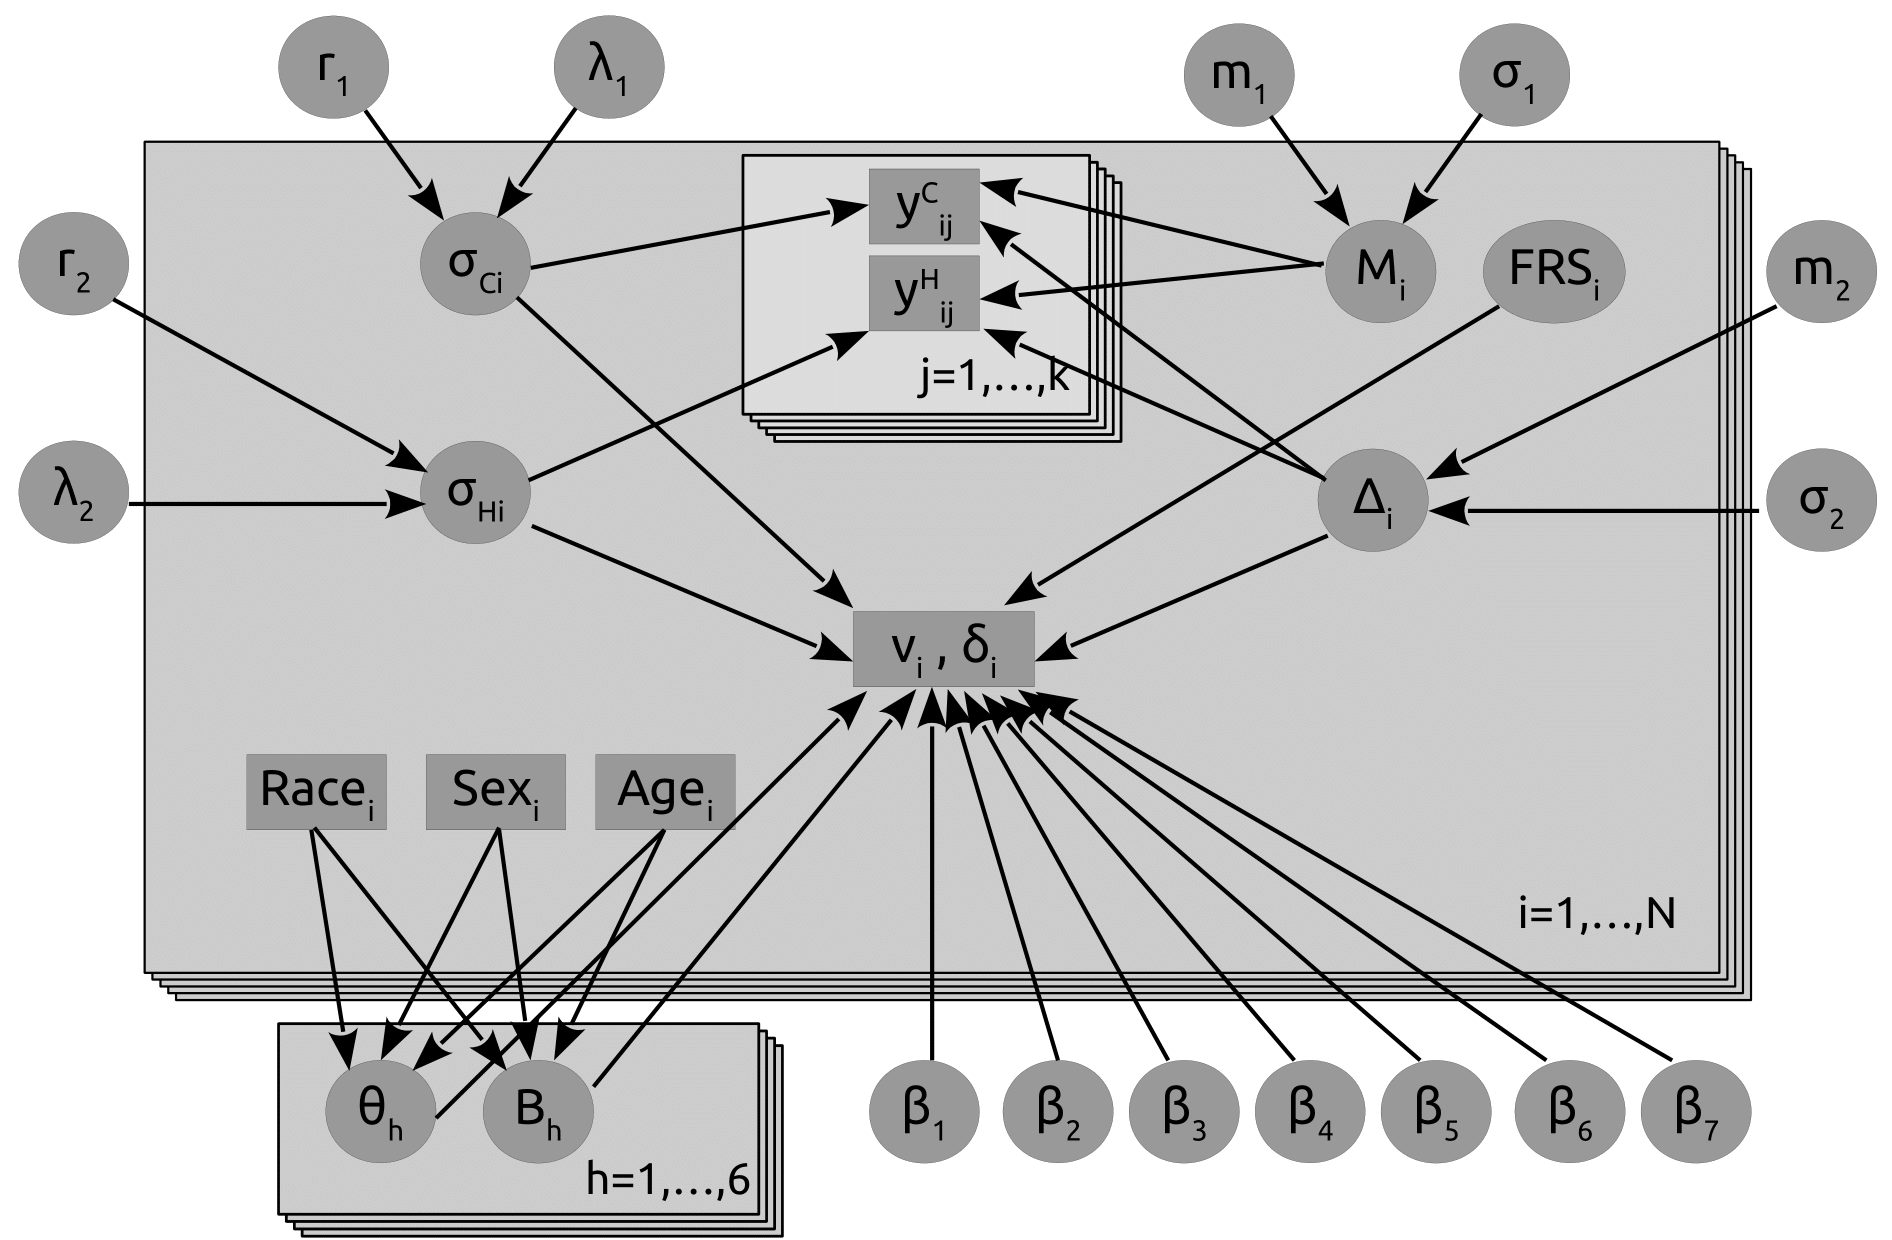
\includegraphics{./DAG_FRS.png}
\caption{An illustration of the DAG of the FRS-based model presented in
this article.}\label{fig:DAGFRS}
}
\end{figure}

\hypertarget{methodology}{%
\subsection{Methodology}\label{methodology}}

The methodology for this research can be split into three main sections:
1) calculating the empirical Bayes' parameters, 2) parameterizing the
model using Hamiltonian Monte Carlo (HMC) and 3) re-centering the
variables in the linear predictor equation. By applying empirical
Bayes', Maximum Likelihood Estimates (MLEs) of some of the parameter
distributions are provided. Note that the parameters estimated here are
only the prior distribution of the global (not individual) blood
pressure means and the variances, for both systolic and diastolic and
home and clinic measurements. These estimates are then provided as prior
distributions for the Stan MCMC simulations using HMC, where estimates
can be made for all the parameter distributions of the model, given the
specific centering applied. Finally, section (3) recalculates the
centering values based on the previous MCMC iteration, and sets of the
next iteration, while simultaneously checking for convergence in both
the MCMC simulations and the centering values.

\hypertarget{empirical-bayes-parameters}{%
\subsubsection{Empirical Bayes
Parameters}\label{empirical-bayes-parameters}}

\hypertarget{extract-intervals-for-the-digits}{%
\subsection{Extract intervals for the
digits}\label{extract-intervals-for-the-digits}}

Suppose the fractions of digits 0,2,4,6,8 are \(b_0,b_2,b_4,b_6,b_8\).
Letting \(B_0=0\) and \(B_k=10\sum_{j=0}^{k-1}b_{2j}\) for
\(k=1,\dots,5\), we want to choose a positive \(a\) and place breaks at
\(-a+B_k\), so that measurements between \(-a+B_k\) and \(-a+B_{k+1}\)
modulo 10 are assigned the final digit \(2k\), for \(k=0,\dots,4\). We
choose \(a\) to minimise the total distance of the intervals from the
rounded value: \[
  \sum_{k=0}^4 \int_{-a+B_k}^{-a+B_{k+1}} \bigl| x-2k\bigr|\mathrm{d} x=\frac12\sum_{k=0}^4 \left(-a+B_k-2k\right)^2 + \left(-a+B_{k+1}-2k\right)^2,
\] as long as \(2k\) is in the appropriate interval. This is minimized
at \[
  a= \frac{1}{5}\left(B_1+B_2+B_3+B_4 - 15\right)=\sum_{j=0}^3 (8-2j) b_{2j} \, - 3.
\]

\hypertarget{fit-the-bp-distribution-parameters}{%
\subsection{Fit the BP distribution
parameters}\label{fit-the-bp-distribution-parameters}}

We suppose that each individual has BP measures \(\tilde{y}_{ij}^l\) for
\(i=1,\dots,n\), \(j=1,\dots,k\) (default \(k=3\)), and \(l=1,2\), which
are rounded versions of \[
  y_{ij}^l \sim \mathcal{N}\bigl( \mu_i^l,(\tau_i^l)^{-1}\bigr),
\] where \begin{align*}
\mu_i^1&=(M_i+\Delta_i)/2,\\
\mu_i^2&=(M_i-\Delta_i)/2,\\
M_i&\sim \mathcal{N}\bigl(m_M,\sigma^2_M) \text{ and }
  \Delta_i\sim \mathcal{N}\bigl(m_\Delta,\sigma^2_\Delta) \text{ independent,}\\
  \tau_i^l &\sim \mathrm{Gamma}(\alpha^l,\alpha^l/\theta^l ).
\end{align*} (Note that \(\alpha^l\) is the usual shape parameter, while
\(\theta^l\) is the expectation.)

We wish to estimate the eight parameters \[
(m_M,m_\Delta,\sigma^2_M,\sigma^2_\Delta,\alpha^1,\theta^1,\alpha^2,\theta^2)
\] We begin by assuming \(y_{ij}^l\) observed directly. We estimate by
maximising the partial likelihood on the observations \begin{align*}
  \bar{y}_{i+}&:= \frac{1}{2k} \sum_{j=1}^k y_{ij}^1 + y_{ij}^2,\\
  \bar{y}_{i-}&:= \frac{1}{2k} \sum_{j=1}^k y_{ij}^1 - y_{ij}^2,\\
  s_i^l&:=  \frac{1}{k-1}\sum_{j=1}^k \Bigl( y_{ij}^l - \frac{1}{k} \sum_{j=1}^k y_{ij}^l \Bigr)^2.
\end{align*} Note that \[
(k-1)s_i^l \tau_i^l =\sum_{j=1}^k \Bigl( z_{ij}^l - \frac{1}{k} \sum_{j=1}^k z_{ij}^l \Bigr)^2.
\] where \(z_{ij}^l\) are i.i.d.~standard normal is independent of
\(\tau_i^l\), thus has a chi-squared distribution with \(k-1\) degrees
of freedom --- hence \(\frac{k-1}{2}\cdot s_i^l\tau_i^l\) is gamma
distributed with parameters \((\frac{k-1}{2},1)\). Since
\(\frac{\alpha}{\theta}\tau_i^l\) is independent of \(s_i^l\tau_i^l\),
with \(\mathrm{Gamma}(\alpha,1)\) distribution, we see that
\(\frac{\theta(k-1)}{2\alpha}s_i^l\) is the ratio of two independent
gamma random variables, hence has beta-prime distribution with
parameters \(\left(\frac{k-1}{2}, \alpha \right)\), so log partial
likelihood \[
  \ell_{\operatorname{Beta}}(\alpha,\theta;s^l_\cdot)=n\alpha \log\frac{\alpha}{\theta}+n\log\Gamma\left(\alpha+\frac{k-1}{2}\right)-n\log\Gamma(\alpha)
  + \frac{k-1}{2} \sum_{i=1}^n \log s_i^l -\left(\alpha+\frac{k-1}{2}\right) \sum_{i=1}^n \log \left(s_i^l+\frac\alpha\theta\right).
\] Note as well that these quantities \((k-1)s_i^l\) should correspond
to empirically observed individual variances; hence we will compare
these empirical variances (with imputed fractional parts) divided by the
normalization factor \(2\alpha/(k-1)\theta\) to the beta-prime
distribution below as a goodness-of-fit test.

The partial Fisher Information has entries \begin{align*}
 -\frac{\partial^2 \ell}{\partial \alpha^2} &=
   n\psi_1\left(\alpha\right) - n\psi_1\left(\alpha+\frac{k-1}{2}\right)
  - \frac{n}{\alpha} +\sum_{i=1}^n \frac{2\theta s_i^l + \alpha-(k-1)/2}{(\theta s_i^l + \alpha)^2}\\
-\frac{\partial^2 \ell}{\partial \theta^2} &=
   -\frac{n \alpha}{\theta^2} +\frac{\alpha}{\theta^2}\left(\alpha+\frac{k-1}{2}\right)\sum_{i=1}^n \frac{2\theta s_i^l + \alpha}{(\theta s_i^l + \alpha)^2}\\
-\frac{\partial^2 \ell}{\partial \theta\partial\alpha} &= \frac{n}{\theta}-
   \frac1\theta \sum_{i=1}^n \frac{\alpha^2+2\alpha\theta s_i^l+\frac{k-1}{2}\theta s_i^l}{(\theta s_i^l + \alpha)^2}.
\end{align*} where \(\psi_1\) is the trigamma function.

Let \((\hat\alpha^l,\hat\beta^l)\) be the maximum partial likelihood
estimators. Conditioned on \((\tau_i^l)\) we have \begin{align*}
  \bar{y}_{i+}&\sim \mathcal{N}\left(m_M, \sigma^2_M + \frac{1}{4k}\left( \frac{1}{\tau_i^1}+\frac{1}{\tau_i^2}\right)\right),\\
  \bar{y}_{i-}&\sim \mathcal{N}\left(m_\Delta,\sigma^2_\Delta + \frac{1}{4k}\left( \frac{1}{\tau_i^1}+\frac{1}{\tau_i^2}\right)\right).
\end{align*} We would then have MLEs \begin{align*}
  \hat{m}_M&= \frac{1}{n} \sum_{i=1}^n \bar{y}_{i+},\\
  \hat{m}_\Delta&= \frac{1}{n} \sum_{i=1}^n \bar{y}_{i-},
\end{align*} which are approximately normally distributed, with means
\(m_M\) and \(m_\Delta\) respectively, and conditional on \(\tau_i^l\)
standard errors \[
  \frac{\sigma_M^2}{n}+\frac{1}{4kn^2} \sum_{i=1}^n (\tau_i^1)^{-1} + (\tau_i^2)^{-1} \quad \text{ and } \quad
  \frac{\sigma_\Delta^2}{n}+\frac{1}{4kn^2} \sum_{i=1}^n (\tau_i^1)^{-1} + (\tau_i^2)^{-1},
\] which we may approximate --- with error on the order of \(n^{-3/2}\)
--- replaceing the mean of \((\tau_i^l)^{-1}\) by its expected value
\(\beta^l/(\alpha^l-1)\) to obtain \begin{align*}
  \mathrm{Var}(\hat{m}_M) &\approx \frac{\sigma_M^2}{n}+\frac{1}{4kn}\left( \frac{\beta^1}{\alpha^1-1}+ \frac{\beta^2}{\alpha^2-1}\right) \\
  \mathrm{Var}(\hat{m}_\Delta) &\approx \frac{\sigma_\Delta^2}{n}+\frac{1}{4kn}\left( \frac{\beta^1}{\alpha^1-1}+ \frac{\beta^2}{\alpha^2-1}\right) 
\end{align*} Finally, conditioned on the \(\tau_i^l\) we have that the
random variables \(\bar{y}_{i+}\) are normal with variance \[
  \sigma_M^2+\frac{1}{4k}\left((\tau_i^1)^{-1} + (\tau_i^1)^{-1} \right),
\] so the unconditional variance is the expected value, or \[
  \sigma_M^2+\frac{1}{4k}\left(\frac{\beta^1}{\alpha^1-1}+ \frac{\beta^2}{\alpha^2-1} \right).
\] This yields the estimators \begin{align*}
  \hat\sigma_M^2 &=\frac{1}{n-1}\sum_{i=1}^n\left(\bar{y}_{i+}-n^{-1}\sum_{i=1}^n y_{i+}\right)^2 - \frac{1}{4k}\left(\frac{\hat\beta^1}{\hat\alpha^1-1}+ \frac{\hat\beta^2}{\hat\alpha^2-1} \right),\\
  \hat\sigma_\Delta^2 &=\frac{1}{n-1}\sum_{i=1}^n\left(\bar{y}_{i-}-n^{-1}\sum_{i=1}^n y_{i-}\right)^2 - \frac{1}{4k}\left(\frac{\hat\beta^1}{\hat\alpha^1-1}+ \frac{\hat\beta^2}{\hat\alpha^2-1} \right).
\end{align*} Using the delta method, and the fact that we see that the
variance of \(\hat\beta/(\hat\alpha-1)\) is approximately \[
  \frac{\sigma_\beta^2}{(\hat\alpha-1)^2} + \frac{\hat\beta^2\sigma_\alpha^2}{(\hat\alpha-1)^4},
\] where \(\sigma_\alpha\) and \(\sigma_\beta\) are the standard errors
for \(\hat\alpha\) and \(\hat\beta\) respectively, so the standard
errors for \(\hat\sigma_M^2\) and \(\hat\sigma_\Delta^2\) are
approximately \begin{align*}
  \operatorname{SE}\left(\hat\sigma_M^2\right)&\approx \frac{1}{2k}\Bigl(\frac{8k^2\hat\sigma_M^2}{n} + \frac{\sigma_\beta^2}{(\hat\alpha^1-1)^2} + \frac{(\hat\beta^1)^2\sigma_\alpha^2}{(\hat\alpha^1-1)^4} + \frac{\sigma_\beta^2}{(\hat\alpha^2-1)^2} + \frac{(\hat\beta^2)^2\sigma_\alpha^2}{(\hat\alpha^2-1)^4} \Bigr)^{1/2},\\
  \operatorname{SE}\left(\hat\sigma_\Delta^2\right)&\approx \frac{1}{2k}\Bigl(\frac{8k^2\hat\sigma_\Delta^2}{n} + \frac{\sigma_\beta^2}{(\hat\alpha^1-1)^2} + \frac{(\hat\beta^1)^2\sigma_\alpha^2}{(\hat\alpha^1-1)^4} + \frac{\sigma_\beta^2}{(\hat\alpha^2-1)^2} + \frac{(\hat\beta^2)^2\sigma_\alpha^2}{(\hat\alpha^2-1)^4} \Bigr)^{1/2}
\end{align*}

\hypertarget{now-compute-the-combined-variance}{%
\subsubsection{Now compute the combined
variance}\label{now-compute-the-combined-variance}}

For a parameter like \(\alpha\) we estimate the variance of
\(\hat\alpha\) by \newcommand{\E}{\mathbb{E}}
\renewcommand{\P}{\mathbb{P}} \[
  \mathrm{Var}(\hat\alpha) = \mathbb{E}\bigl[ \mathrm{Var}\left(\hat\alpha\, |\, I\right)\bigr] + \mathrm{Var}\left(\mathbb{E} \left[ \hat\alpha\, |\, I \right]\right).
\] Here \(I\) represents the randomly imputed fractional part. We can
estimate the first term by averaging the estimated variance (from Fisher
Information) over all random imputations. We estimate the second term by
the variance of the \(\alpha\) estimates over imputations. Note that
this is not quite right, since what we really want the variance of is
\(\alpha_0(I)\) --- effectively, the ``true'\,' parameter consistent
with the imputation. This is a plug-in estimate, as is the Fisher
Information estimate of the variance.

\hypertarget{computing-residuals}{%
\subsection{Computing residuals}\label{computing-residuals}}

We define the deviance for an individual \(i\) with observations
\((Y_i)\) given the hyperparameters
\(h=(m_M,m_\Delta,\sigma^2_M,\sigma^2_\Delta,\alpha^H,\theta^H,\alpha^C,\theta^C)\)
\[
  D= \sum_{i=1}^n \log \mathbb{P}\left\{ \mathbf{Y}_{i}\,|\, \text{hyperparameters}=h\right\}.
\] \newcommand{\wtb}{\widetilde\mathbf} Since the \(\mathbf{Y}_i\) are
independent conditioned on \(h\), \begin{align*}
D&= \sum_{i=1}^n \log \mathbb{E}_h\left[ \mathbb{P}\left\{ \mathbf{Y}_i \, |\, M_i,\Delta_i,\tau_i^{C},\tau_i^H \right\} \right]\\
    &\approx \sum_{i=1}^n \log \frac1R\sum_{r=1}^R \left[ \mathbb{P}\left\{ \mathbf{Y}_i \, |\, M_{i,r},\Delta_{i,r},\tau_{i,r}^{C},\tau_{i,r}^{H} \right\}\right] \frac{\pi_h(M_{i,r},\Delta_{i,r},\tau_{i,r}^{C},\tau_{i,r}^{H} )}{q(M_{i,r},\Delta_{i,r},\tau_{i,r}^{C},\tau_{i,r}^{H} \, | \, h,\, \mathbf{Y}_i)},
\end{align*} where
\((M_{i,r},\Delta_{i,r},\tau_{i,r}^{C},\tau_{i,r}^{H})\) are independent
samples from a distribution \(q\) that may depend on \(\mathbf{Y}_i\)
and \(h\), and \(\pi_h\) is the true density of those individual
parameters given hyperparameters \(h\).

\hypertarget{check-variance-distribution-empirically}{%
\subsubsection{Check variance distribution
empirically}\label{check-variance-distribution-empirically}}

We wish to check whether the continuous distribution we have fit for
individual variances describes the true distribution of variances in the
population reasonably well. The first thing we do is to compare the
empirical variances (with imputed fractional parts) to the theoretical
beta-prime distribution. To match the standard distribution, the
variances are normalized by being divided by the factor
\(\alpha/\theta\). Note that the distribution has a very long tail, and
we have truncated the plot at a point where about

\begin{verbatim}
## NULL
\end{verbatim}

\begin{verbatim}
## Warning: The dot-dot notation (`..density..`) was deprecated in ggplot2 3.4.0.
## i Please use `after_stat(density)` instead.
\end{verbatim}

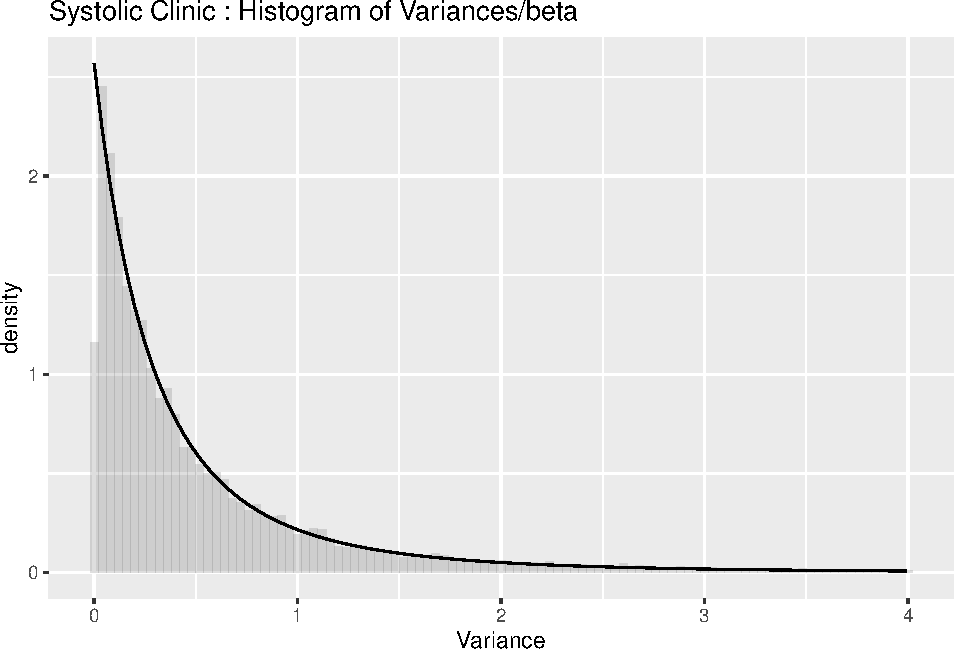
\includegraphics{Appendix_files/figure-latex/Variance test-1.pdf}

\begin{verbatim}
## NULL
\end{verbatim}

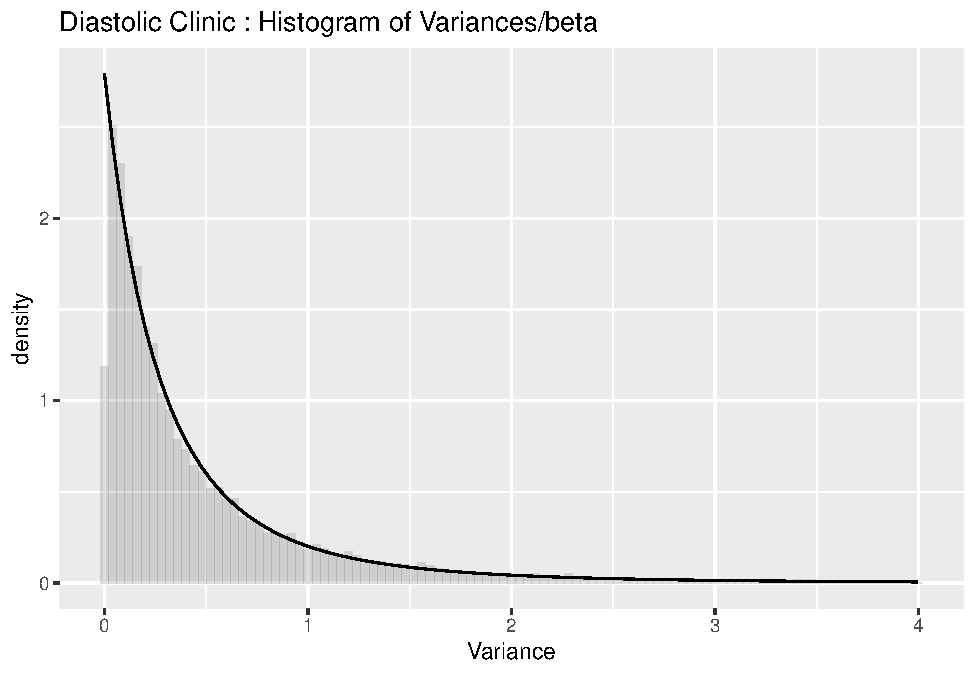
\includegraphics{Appendix_files/figure-latex/Variance test-2.pdf} Now we
generate data from the inferred model that mimic the true data, with
three systolic and three diastolic BP measures per person. These cannot
be directly compared with the observed data, which are rounded to the
nearest 2 (in a somewhat biased way), so we randomly impute the
fractional part, which we add to the true observations. This gives us a
set of true variances and a set of simulated variances, which we hope
will have approximately the same distribution. We compare these --- for
each of the four combinations of systolic/diastolic and home/clinic ---
by Q--Q plots.

\begin{verbatim}
## Warning: Multiple drawing groups in `geom_function()`
## i Did you use the correct group, colour, or fill aesthetics?
\end{verbatim}

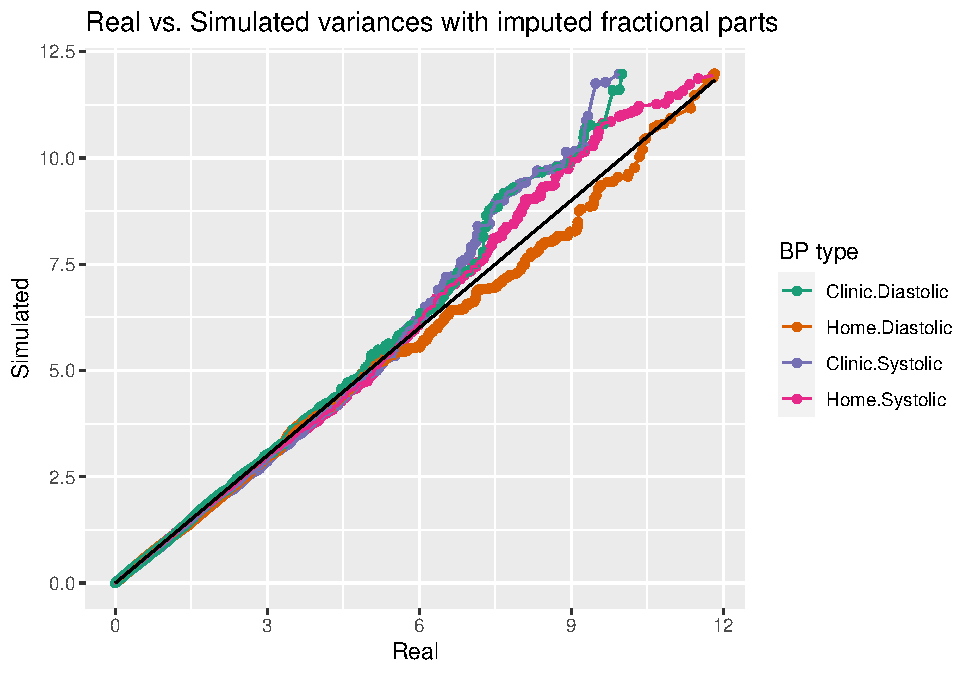
\includegraphics{Appendix_files/figure-latex/Compare variances-1.pdf}

\hypertarget{hamiltonian-monte-carlo-hmc}{%
\subsubsection{Hamiltonian Monte Carlo
(HMC)}\label{hamiltonian-monte-carlo-hmc}}

The model, as described in the article, is a Bayesian hierarchical
model. In order to parameterize such an intricate model, traditional
Maximum Likelihood Estimation methods can no longer be applied.
Therefore, we apply the Hamiltonian Monte Carlo (HMC) method. HMC is a
form of Markov Chain Monte Carlo methods, which samples potential
parameter space values of the model, then calculates directly the
likelihood function based on that choice of parameters. The derivative
of the likelihood function, \(\phi\), guides parameter space exploration
in \(\theta\) towards the modal value of the joint posterior
distribution. This method is ideal for complicated, non-Gaussian
distribution forms. The three steps of HMC are:

\begin{enumerate}
\item Draw a sample of the derivative $\phi$ using the posterior distribution of $\phi$, which is the same as its prior.
\item Update the values of $\theta^*$ and $\phi^*$ using
  \begin{equation}
    \theta^*\leftarrow \theta+\epsilon M^{-1}\phi,
  \end{equation}
  and
  \begin{equation}
    \phi\leftarrow \phi+\epsilon\frac{1}{2}\frac{d\log\{p(\theta|y)\}}{d\theta},
  \end{equation}
where $M$ is the jacobian of the parameters. This can be set to a diagonal matrix for no correlation between parameters, and is pointwise updated throughout the calculation. This is the leapfrog method, whereby $\epsilon$ dictates the scale size of the step to ensure convergence on the correct point is made, and L is the number of steps to be `leaped'.
\item Compute the rejection parameter:
  \begin{equation}
    r=\frac{p(\theta^*|y)p(\phi^*)}{p(\theta^{t-1}|y)p(\phi^{t-1})}
  \end{equation}
\item Set $\theta^t$ to $\theta^*$ with probability $\min\{1,r\}$, or otherwise keep $\theta^{t-1}$.
\end{enumerate}

The tuning parameters \(\epsilon\) and L should be chosen according to a
desired acceptance rate. The No-U-Turn Sampler of Stan automates the
calculation of these tuning parameters. A more detailed overview of HMC
and the NUTS algorithm integrated into the Stan package, see \emph{`The
No-U-Turn Sampler: Adaptively Setting Path Lengths in Hamiltonian Monte
Carlo'} by M. Hoffman and A. Gelman, Journal of Machine Learning
Research, 15, 1351-1381 (2014).

\hypertarget{centering-the-linear-predictor}{%
\subsubsection{Centering the Linear
Predictor}\label{centering-the-linear-predictor}}

During the MCMC simulations, the centering values play a non-negligible
role in shaping the model parameterization. If the centering parameters
are held constant throughout all of the MCMC simulations, then the
equation
\(\sum_i^N \exp{(\boldsymbol{\beta}\cdot(\boldsymbol{X}-\hat{X}))}=0\)
is no longer guaranteed. However, automatically defining the centering
values based on the model parameters sampled at the current MCMC
iteration is not advisable as it can lead to poor parameter convergence.
This is because it modifies the likelihood function at every MCMC
iteration. Therefore, we iterate the MCMC algorithm multiple times. At
every iteration, we recalculate the centering parameters to satisfy the
requirement that the average of the linear predictor term going to zero,
based on the posterior distributions of the previous MCMC simulation.
This iteration is carried out until the centering parameters converge.
Convergence is defined by optimising on two factors. The first is that
the sum of the linear predictor term across all MCMC samples needs to
tend to negligible values (we define this as the average difference
being less than \(10^{-7}\)), see figure \ref{fig:linpred_conv}. The
second convergence criteria is that the average Root Mean-Squared Error
(RMSE) of the model predictions on the survival outcomes in the MCMC
simulations needs to also decrease towards zero, see figure
\ref{fig:linpred_conv} (top). For the second criteria, we stopped the
simulations when either the difference in the RMSE stopped decreasing
(below a threshold of \(1\%\)), or the RMSE value was less than 20, see
figure \ref{fig:linpred_conv} (bottom). Illustration of the convergence
is shown in figure \ref{fig:linpred_conv}.

\hypertarget{code-description}{%
\subsection{Code Description}\label{code-description}}

The code can be found at \url{https://github.com/hamishwp/Nhanes2021}.
The numerical code has been built in multiple stages. Below, we explain
the principal files required to replicate the entire analysis presented
in the article. There are 5 main groups for the code:

\begin{enumerate}
\def\labelenumi{\arabic{enumi}.}
\tightlist
\item
  Data cleaning scripts
\item
  Main file
\item
  Stan files for HMC
\item
  Centering recalculation scripts
\item
  Post-processing analysis
\end{enumerate}

We provide a brief description of each of these below.

\hypertarget{data-cleaning}{%
\subsubsection{Data Cleaning}\label{data-cleaning}}

This is found in the file \texttt{Dataclean2021.R}. Provided the raw
NHANES dataset (in CSV format), it extracts all the data required for
the simulations, and stores it in a structure that can be directly read
in to the main file (\texttt{MCMC\_DiasSyst\_v3.R}) of this research.

\hypertarget{main}{%
\subsubsection{Main}\label{main}}

The main file is \texttt{MCMC\_DiasSyst\_v3.R}. It reads in the cleaned
NHANES data, the specific choice of simulation parameters (for example,
whether to use the FRS number or mean systolic \& diastolic blood
pressure), and runs the correct RStan scripts for that specific
selection of simulation parameters. This script is intended for use on
computing clusters.

\hypertarget{stan}{%
\subsubsection{Stan}\label{stan}}

There are eight Stan files:

\begin{enumerate}
\def\labelenumi{\arabic{enumi}.}
\tightlist
\item
  \texttt{mystanmodel\_DS\_sigma\_v2\_autopred.stan}
\item
  \texttt{mystanmodel\_DS\_tau\_v2\_autopred.stan}
\item
  \texttt{mystanmodelFRS\_DS\_sigma\_v2\_autopred.stan}
\item
  \texttt{mystanmodelFRS\_DS\_tau\_v2\_autopred.stan}
\item
  \texttt{mystanmodel\_DS\_sigma\_v2.stan}
\item
  \texttt{mystanmodel\_DS\_tau\_v2.stan}
\item
  \texttt{mystanmodelFRS\_DS\_sigma\_v2.stan}
\item
  \texttt{mystanmodelFRS\_DS\_tau\_v2.stan}
\end{enumerate}

These correspond to the following alternative simulation parameters:

\begin{itemize}
\tightlist
\item
  For the blood-pressure variability, choosing to use the
  standard-deviation \(\sigma\) or the precision \(\tau=1/\sigma\){]}\}
\item
  Using the FRS score or the mean diastolic and systolic blood pressure
  as a covariate in the analysis
\item
  Whether the centering parameters, \(\hat{X}\), in the linear predictor
  term are automatically calculated to satisfy
  \(\sum_i^N \exp{(\boldsymbol{\beta}\cdot(\boldsymbol{X}-\hat{X}))}=0\)
  for every MCMC iteration, or whether the centering is held constant
  across all iterations
\end{itemize}

\hypertarget{centering}{%
\subsubsection{Centering}\label{centering}}

The centering of the linear predictors, which is required as input to
every MCMC simulation iteration, is recalculated in the files
\texttt{AutoPred\_Recalc.R} and \texttt{ManPred\_Recalc.R}. This is then
provided to the Main script, \texttt{MCMC\_DiasSyst\_v3.R}, which
provides these centering values to the Stan code for the MCMC
simulations.

\hypertarget{empirical-bayes-estimation}{%
\subsubsection{Empirical Bayes
Estimation}\label{empirical-bayes-estimation}}

The file \texttt{gamma\_fits.Rmd} contains all the necessary routines in
order to replicate the calculation of the empirical Bayes' priors for
the hyperparameters of the model.

\#\#\#Post-processing The post-processing script is called
\texttt{PostProcessing.R}, which heavily relies on the
\texttt{Functions.R} script which contains all the necessary functions
to analyse the data. The post-processing script generates many useful
plots of the MCMC posterior distribution for the user, including Bayes'
factors, violin plots of the normalised beta and gompertz posteriors,
and more.

\hypertarget{results}{%
\subsection{Results}\label{results}}

In this section, we add some additional detail to the results section
covered in the article. Extra information is given to explain how
convergence of the simulations was ensured, and to also include more
visualisations of the converged model parameterizations. The authors
feel that this is particularly useful to provide confidence in the model
parameterization and the predictions.

\hypertarget{convergence-of-simulations}{%
\subsubsection{Convergence of
Simulations}\label{convergence-of-simulations}}

Convergence of the simulations required to parameterize the model
presented in this work is required for the MCMC simulations performed by
Stan, as well as convergence in the centering values that requires
repeating the Stan calculations several times. Convergence of the latter
is shown in figure \ref{fig:linpred_conv}. The upper plot in figure
\ref{fig:linpred_conv} illustrates convergence in the average Root
Mean-Squared Error (RMSE) of the model predictions on the survival
outcomes in the MCMC simulations. The lower plot in figure
\ref{fig:linpred_conv} illustrates convergence in the average sum of the
linear predictor terms over all MCMC chain iterations.

\begin{figure}
\hypertarget{fig:linpred_conv}{%
\centering
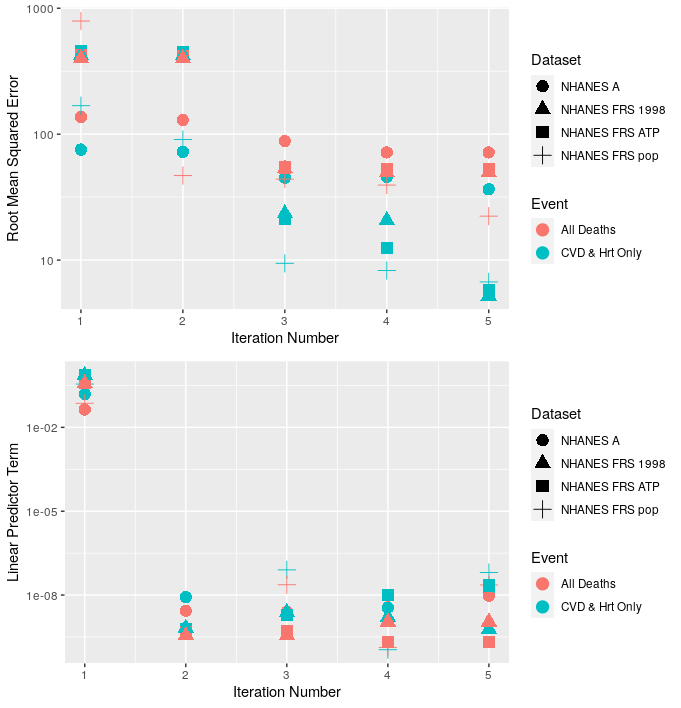
\includegraphics{./Plots/xhat/RMSE-Linpred_Convergence.png}
\caption{Illustration of the convergence of the centering parameters of
the model.}\label{fig:linpred_conv}
}
\end{figure}

With respect to convergence of the MCMC simulations, defining
convergence first involves discarding the burn-in period of the
simulations. When the time-evolution marker chain has a large number of
samples, sequence thinning is used to reduce the amount of data storage
- after convergence, take only the kth value of the simulations (after
having discarded the burn-in phase values) and discard the rest. One
measure of convergence is to bin similar markers and check that for each
bin, the variation of the individual marker movement over a few time
steps is larger than the variation of the ensemble markers in-between
one-another. Other methods of convergence are stationarity and mixing.
The former occurs by ensuring that the gradients of movements in the
chains in time are in the same direction, the latter ensures that the
amplitude of the movements in the chains are similar. To calculate the
mixing and stationarity, one can do the following:

\begin{itemize}
\item Take the proposedly converged marker population, where there are N markers in total each of index length $\tau$ (thus of total physical time quantity $t\tau$). Split it k times, where k is a common denominator of $\tau$.
\item Now you have $kN$ MCMC chains each of length $|\tau/k|$
\item For the marker $\psi_{ij}$ with i and j the chain length (time) and marker number indices respectively, then the mean marker value over the chain length (time) is
  \begin{equation}
    \bar{\psi}_{|,j}=\frac{k}{\tau}\sum_{i=1}^{\tau/k}\psi_{ij}
  \end{equation}
  and the total average quantity of $\psi$ over all markers, over all chain lengths is therefore
  \begin{equation}
    \bar{\psi}_{||}=\frac{1}{kN}\sum_{j=1}^{kN}\bar{\psi}_{|j}
  \end{equation}  
\item Stationarity: compare the inter-marker variance (between sequence B):
  \begin{equation}
    B = \frac{\tau}{k(kN-1)}\sum_{j=1}^{kN}(\bar{\psi}_{|,j}-\bar{\psi}_{||})^2
  \end{equation}
\item Mixing: compare the variance along each markers chain length (within-sequence W):
  \begin{equation}
    W = \frac{1}{n(\tau-k)}\sum_{j=1}^{kN}\sum_{i=1}^{\tau/k}(\psi_{i,j}-\bar{\psi}_{|j})^2
  \end{equation}
\item Therefore, to estimate the marginal posterior variance of $p(\psi|y)$, then we use a weighted average
  \begin{equation}
    \hat{\text{Var}}^+(\psi|y)=\frac{\tau-k}{N}W+\frac{1}{Nk}B
  \end{equation}
  Note that this quantity overestimates the marginal posterior variance, but it is unbiased under stationarity: this can be used to infer convergence. When the varation in
  \begin{equation}
    \hat{R}=\sqrt{\frac{\hat{\text{Var}}^+(\psi|y)}{W}}
  \end{equation}
  should approach close to 1 for converged simulations.
\end{itemize}

Another convergence parameter is the number of effective independent
marker draws. Upon convergence, the time evolution of each marker should
be uncorrelated and independent to previous time steps. To find the
average time-correlation over all particles, we use the variogram
\(V_t\): \begin{equation}
  V_t=\frac{1}{Nk(\tau/k-\tilde{t})}\sum_{j=1}^{kN}\sum_{i=1}^{\tau/k}(\psi_{i,j}-\psi_{i-\tilde{t},j})^2,
\end{equation} where \(\tilde{t}\in 1,2,...,\tau/k\) is a time index.
Then we get the time-correlations: \begin{equation}
  \hat{\rho}_t=1-\frac{V_t}{2\hat{\text{Var}}^+}
\end{equation} This comes from the expectation of the variance
\(E[(\psi_i-\psi_{i-t})^2]=2(1-\rho_t)\text{Var}(\psi)\). This can be
used to infer the effective number of independent marker draws:
\begin{equation}
  \hat{n}_{eff}=\frac{mn}{1+2\sum_{\tilde{t}=1}^T\hat{\rho}_t}
\end{equation} Where T is the index at which the sum of the
autocorrelation estimates \(\hat{\rho}_{t'}+\hat{\rho}_{t'+1}\) is
negative. As a general guide, we should have \(\hat{n}_{eff}\sim 10N/k\)
effective independent marker draws and that \(\hat{R}\to 1\sim 1.1\). In
this research, we continued running the MCMC simulations until these two
criteria were met (and went beyond: \(\hat{R}<1.05\) for all parameters
in all models and that \(\hat{n}_{eff}>750\) for all parameters in all
models).

\hypertarget{results---model-parameterization}{%
\subsubsection{Results - Model
Parameterization}\label{results---model-parameterization}}

We remind the reader of the list of numbers of the different models
explored in this research, provided in the list found in section
`Proposed Models'. The authors will use the numbers in the list,
referred to as the run number, in the following plots. One of the most
important set of parameters of the model is the vector \(\beta\) of
covariates in the Cox' proportional hazards model. When the \(\beta\)
vector is normalised, the larger (in absolute terms) the value of
\(\beta\), the larger the correlation between that specific covariate
and the risk of mortality. Positive values of \(\beta\) imply a higher
risk of mortality, and the inverse for negative values of \(\beta\). As
we can see from the violin plots of the MCMC posterior samples of the
\(\beta\) parameters in figure \ref{fig:betas}, the parameter that
correlated the highest with both the mortality risk of CVD and for all
mortalities, in absolute terms, was the 1998 version of the FRS score,
shown in the top-right plot under run numbers 7 and 8. The FRS-1998
score correlated, on average over all the MCMC iterations, approximately
\(25\%\) more with mortality risk of CVD than the (more recently
developed) FRS ATP III score. A similar, but slightly weaker,
correlation was found between the two FSR scores for all mortality-based
risk. The middle-left plot in figure \ref{fig:betas} shows that the mean
diastolic blood pressure acts to decrease mortality risk. Finally, the
influence of the longer-term difference in the mean blood pressure,
displayed in the top-left and top-middle plots of figure
\ref{fig:betas}, is also shown to increase mortality risk across all run
numbers. The influence of the blood-pressure variability on mortality is
illustrated to not be consistent across simulations, whereby the
statistical significance of the effect is lower than for the other
parameters in the linear predictor term.

\begin{figure}
\hypertarget{fig:betas}{%
\centering
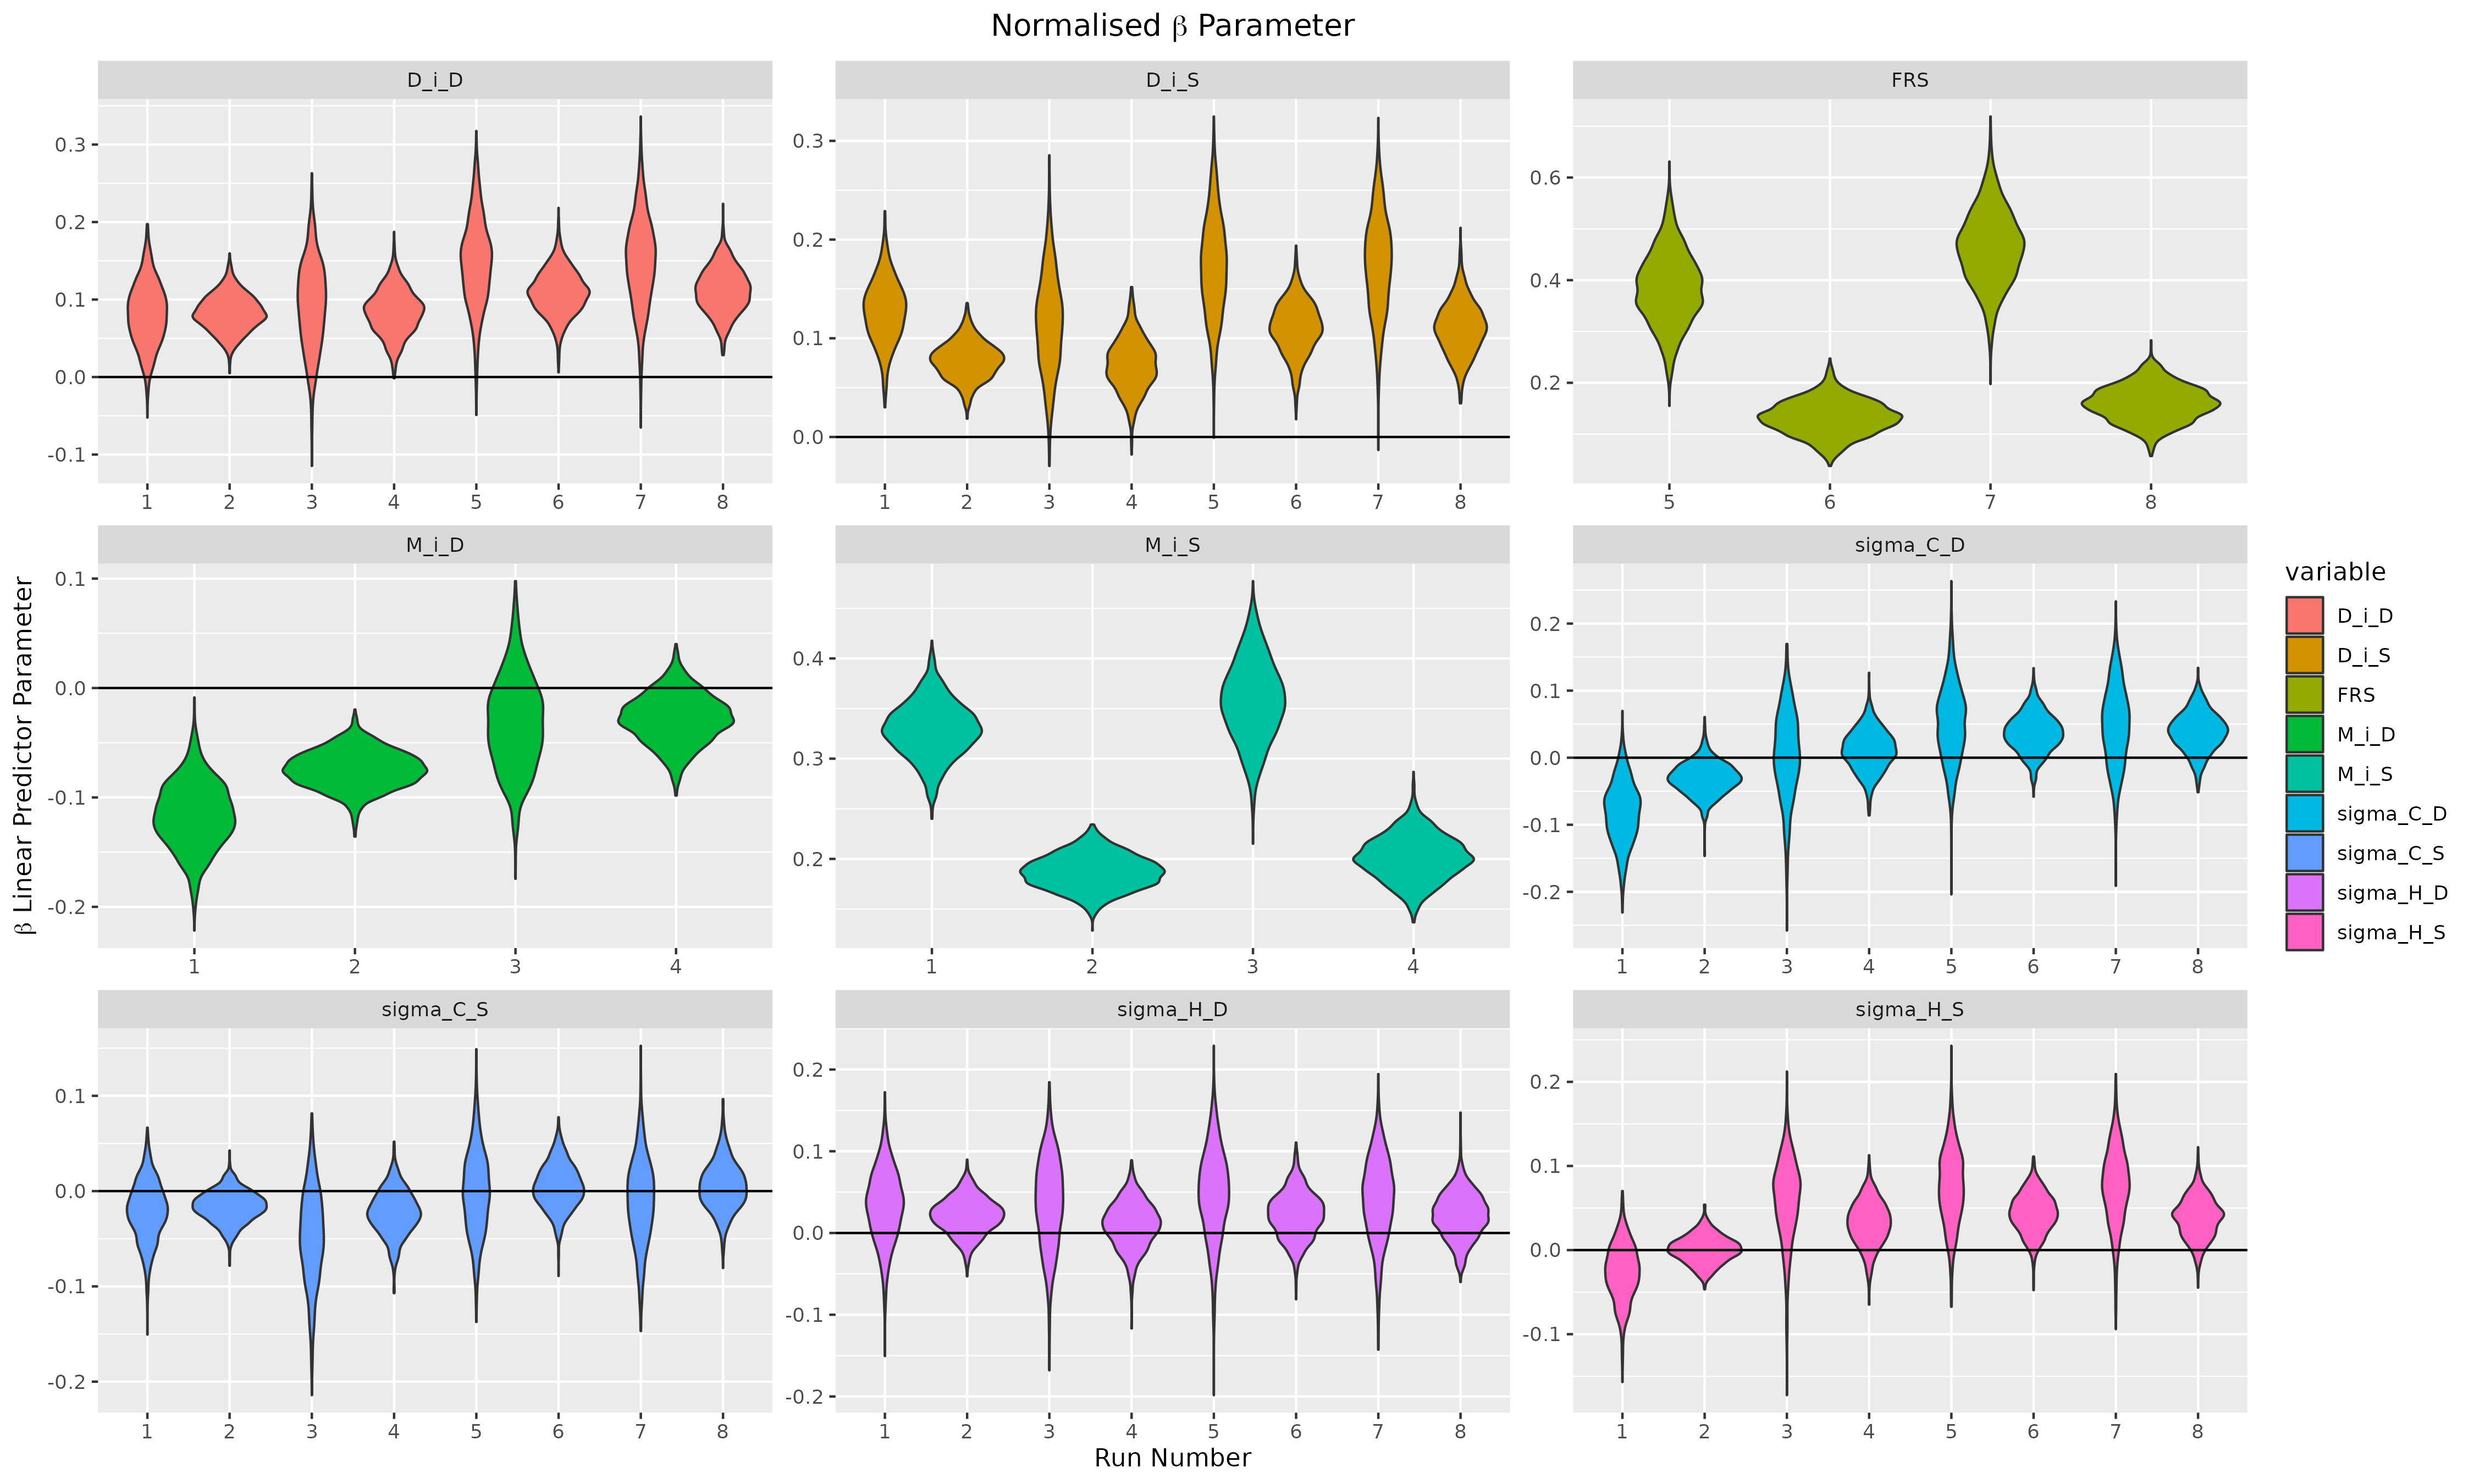
\includegraphics{./Plots/beta/Beta_parameter_normalised.png}
\caption{Violin plots of the normalised \(\beta\) parameters of the
different models.}\label{fig:betas}
}
\end{figure}

With respect to the time-independent Gompertz parameter, described using
\(B\) in this article, the results between all models that simulate CVD
mortality risk, and all the models that simulation all-cause mortality
risk are consistent with one-another. This is illustrated by the
similarity between plots on the left hand side and the right hand side
of figure \ref{fig:gompB}. The consistency appears across sex assigned
at birth and race.

\begin{figure}
\hypertarget{fig:gompB}{%
\centering
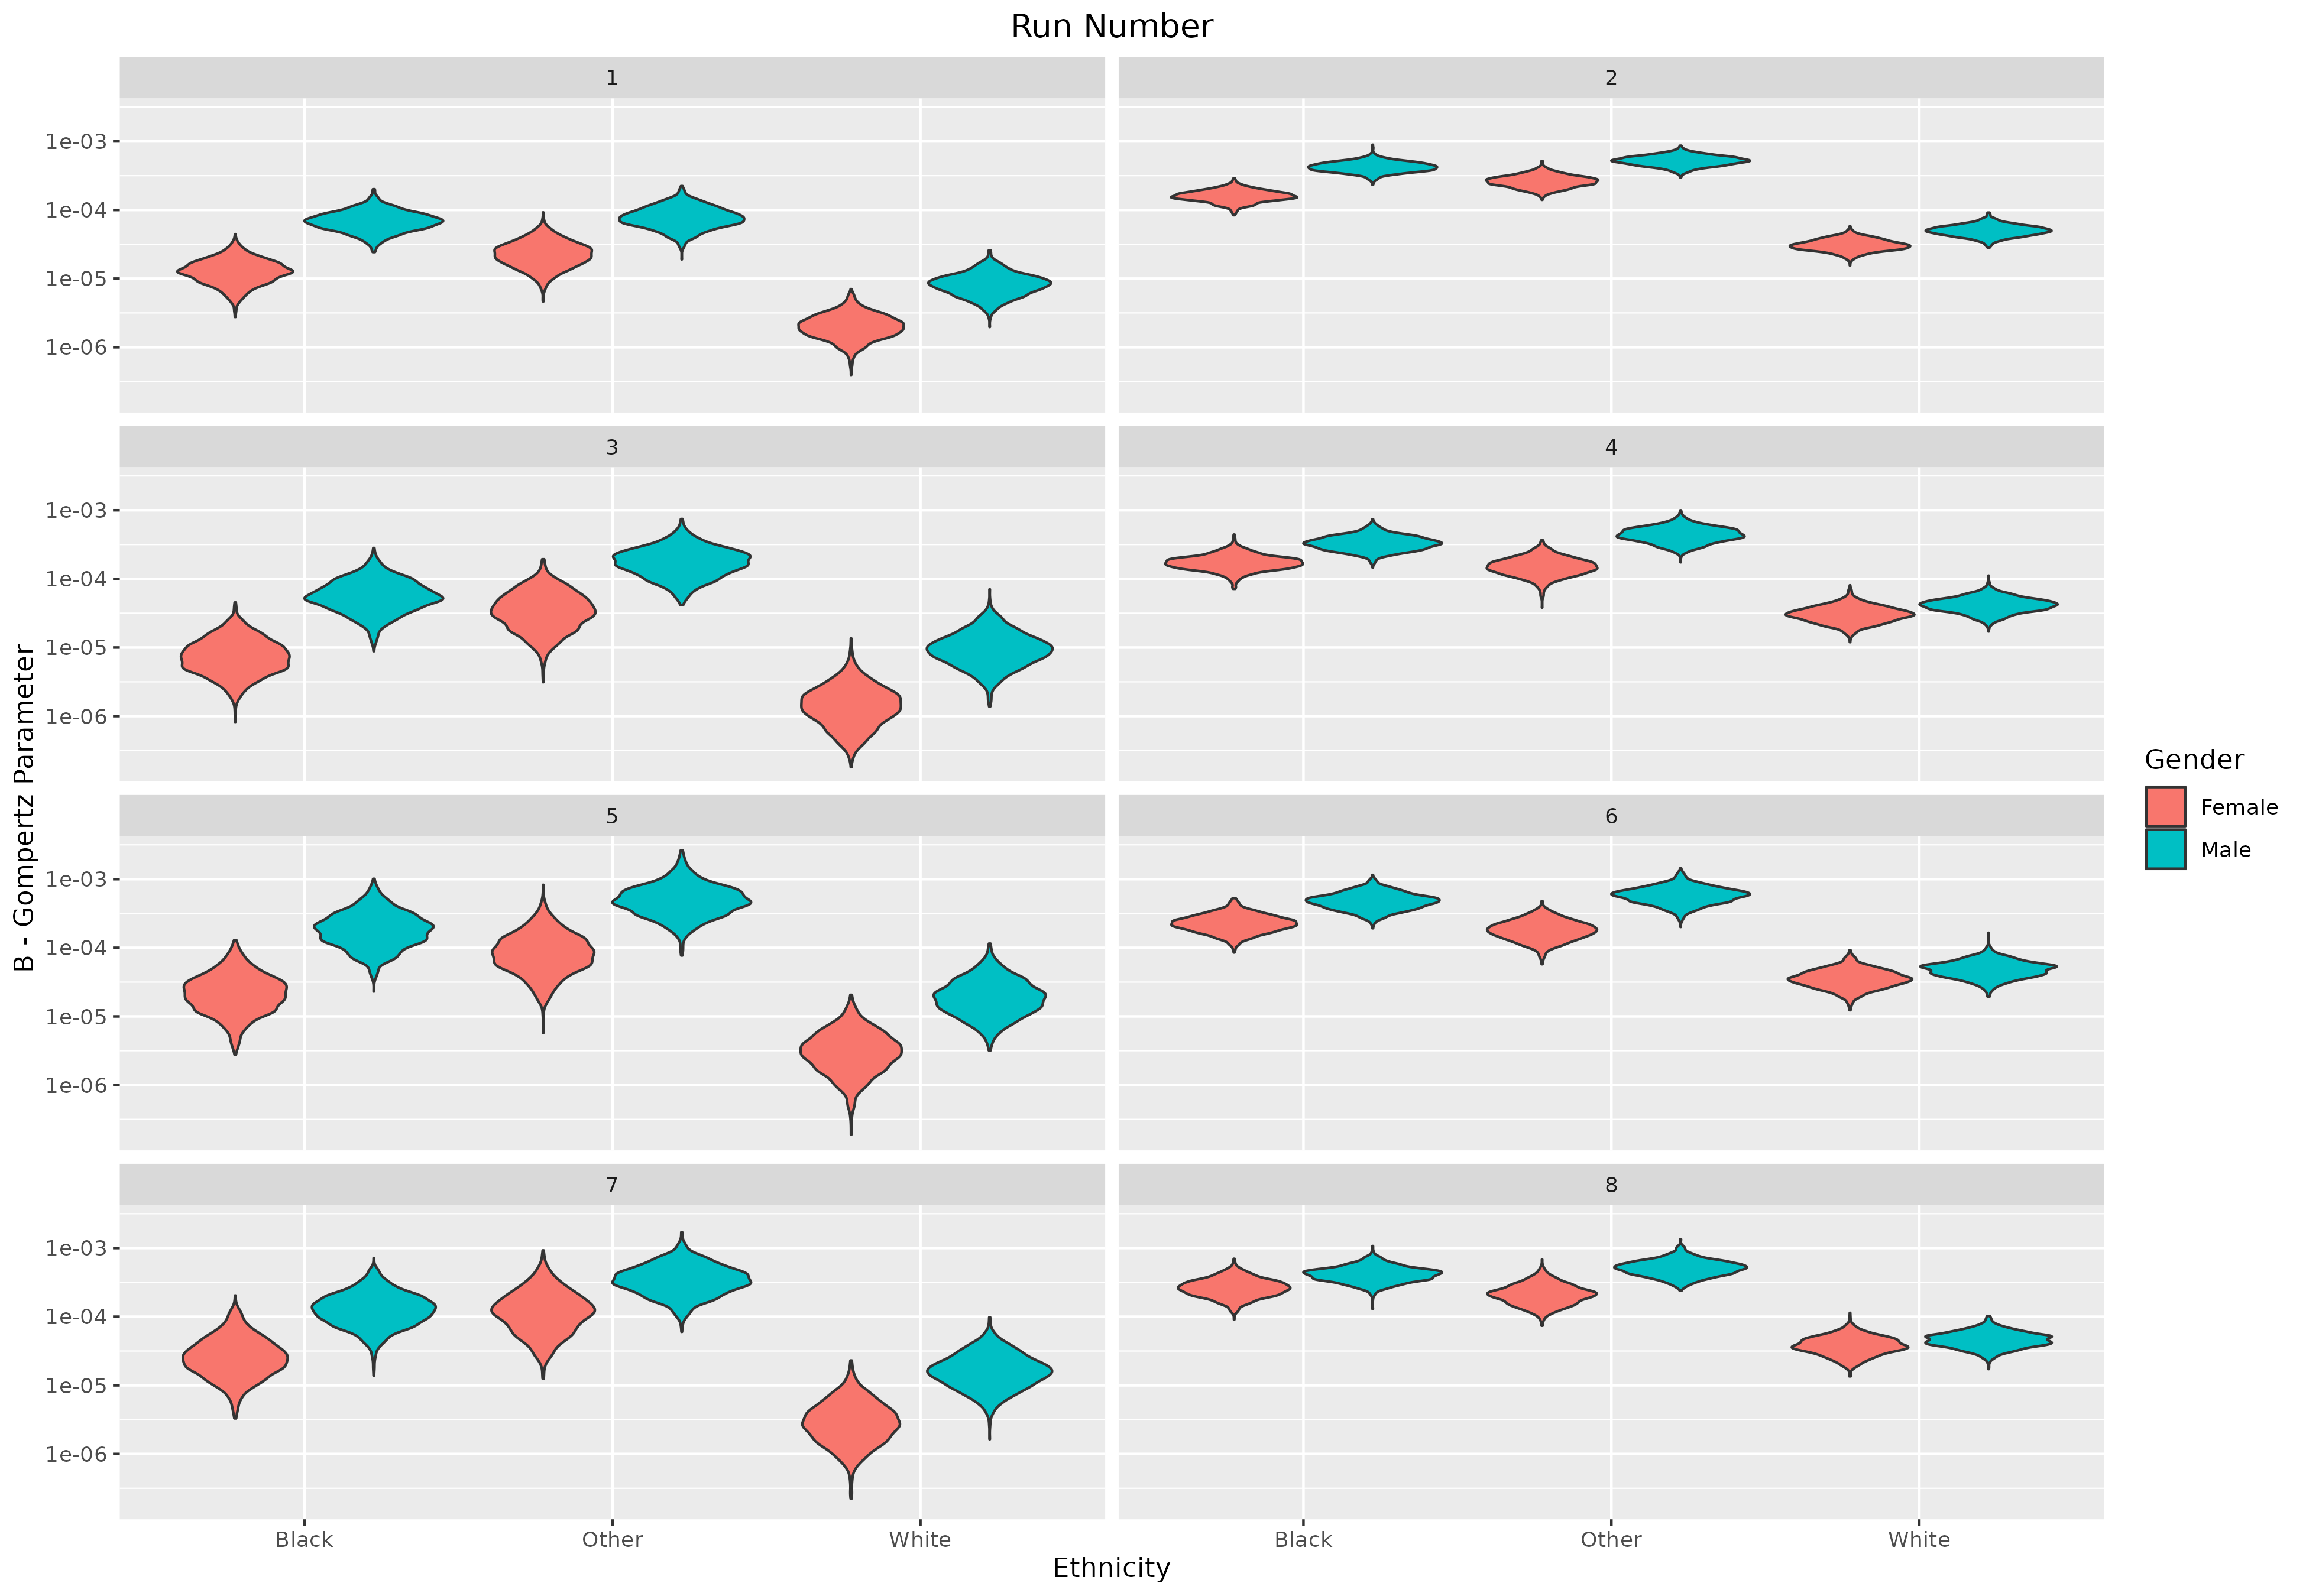
\includegraphics{./Plots/gompertz/B_parameter.png}
\caption{Violin plots of the normalised B parameter (from the Gompertz
equation) of the different models.}\label{fig:gompB}
}
\end{figure}

Figure \ref{fig:gompt} reflects the same level of consistency for the
Gompertz parameter that influences the temporal evolution of the
mortality risk. It is worth noting that both figures \ref{fig:gompB} and
\ref{fig:gompt} have inverse trends between the values of B and theta
for each demographic group. This makes it difficult to imagine, based on
these two plots, what the mortality risk is at different ages across
demographics, yet it is evident that the form of the change in the
mortality risk curve in time is different for each demographic group.
Women are observed to have lower initial values of risk, but mortality
risk later in life begins to increase much faster than for men.
Additionally, hispanic populations are shown to have a larger initial
mortality risk than black populations who are shown to have a larger
initial mortality risk than white populations in the USA. However,
mortality risk increases at a faster rate for white populations than for
black populations, for which it increases faster than hispanic
populations in the USA.

\begin{figure}
\hypertarget{fig:gompt}{%
\centering
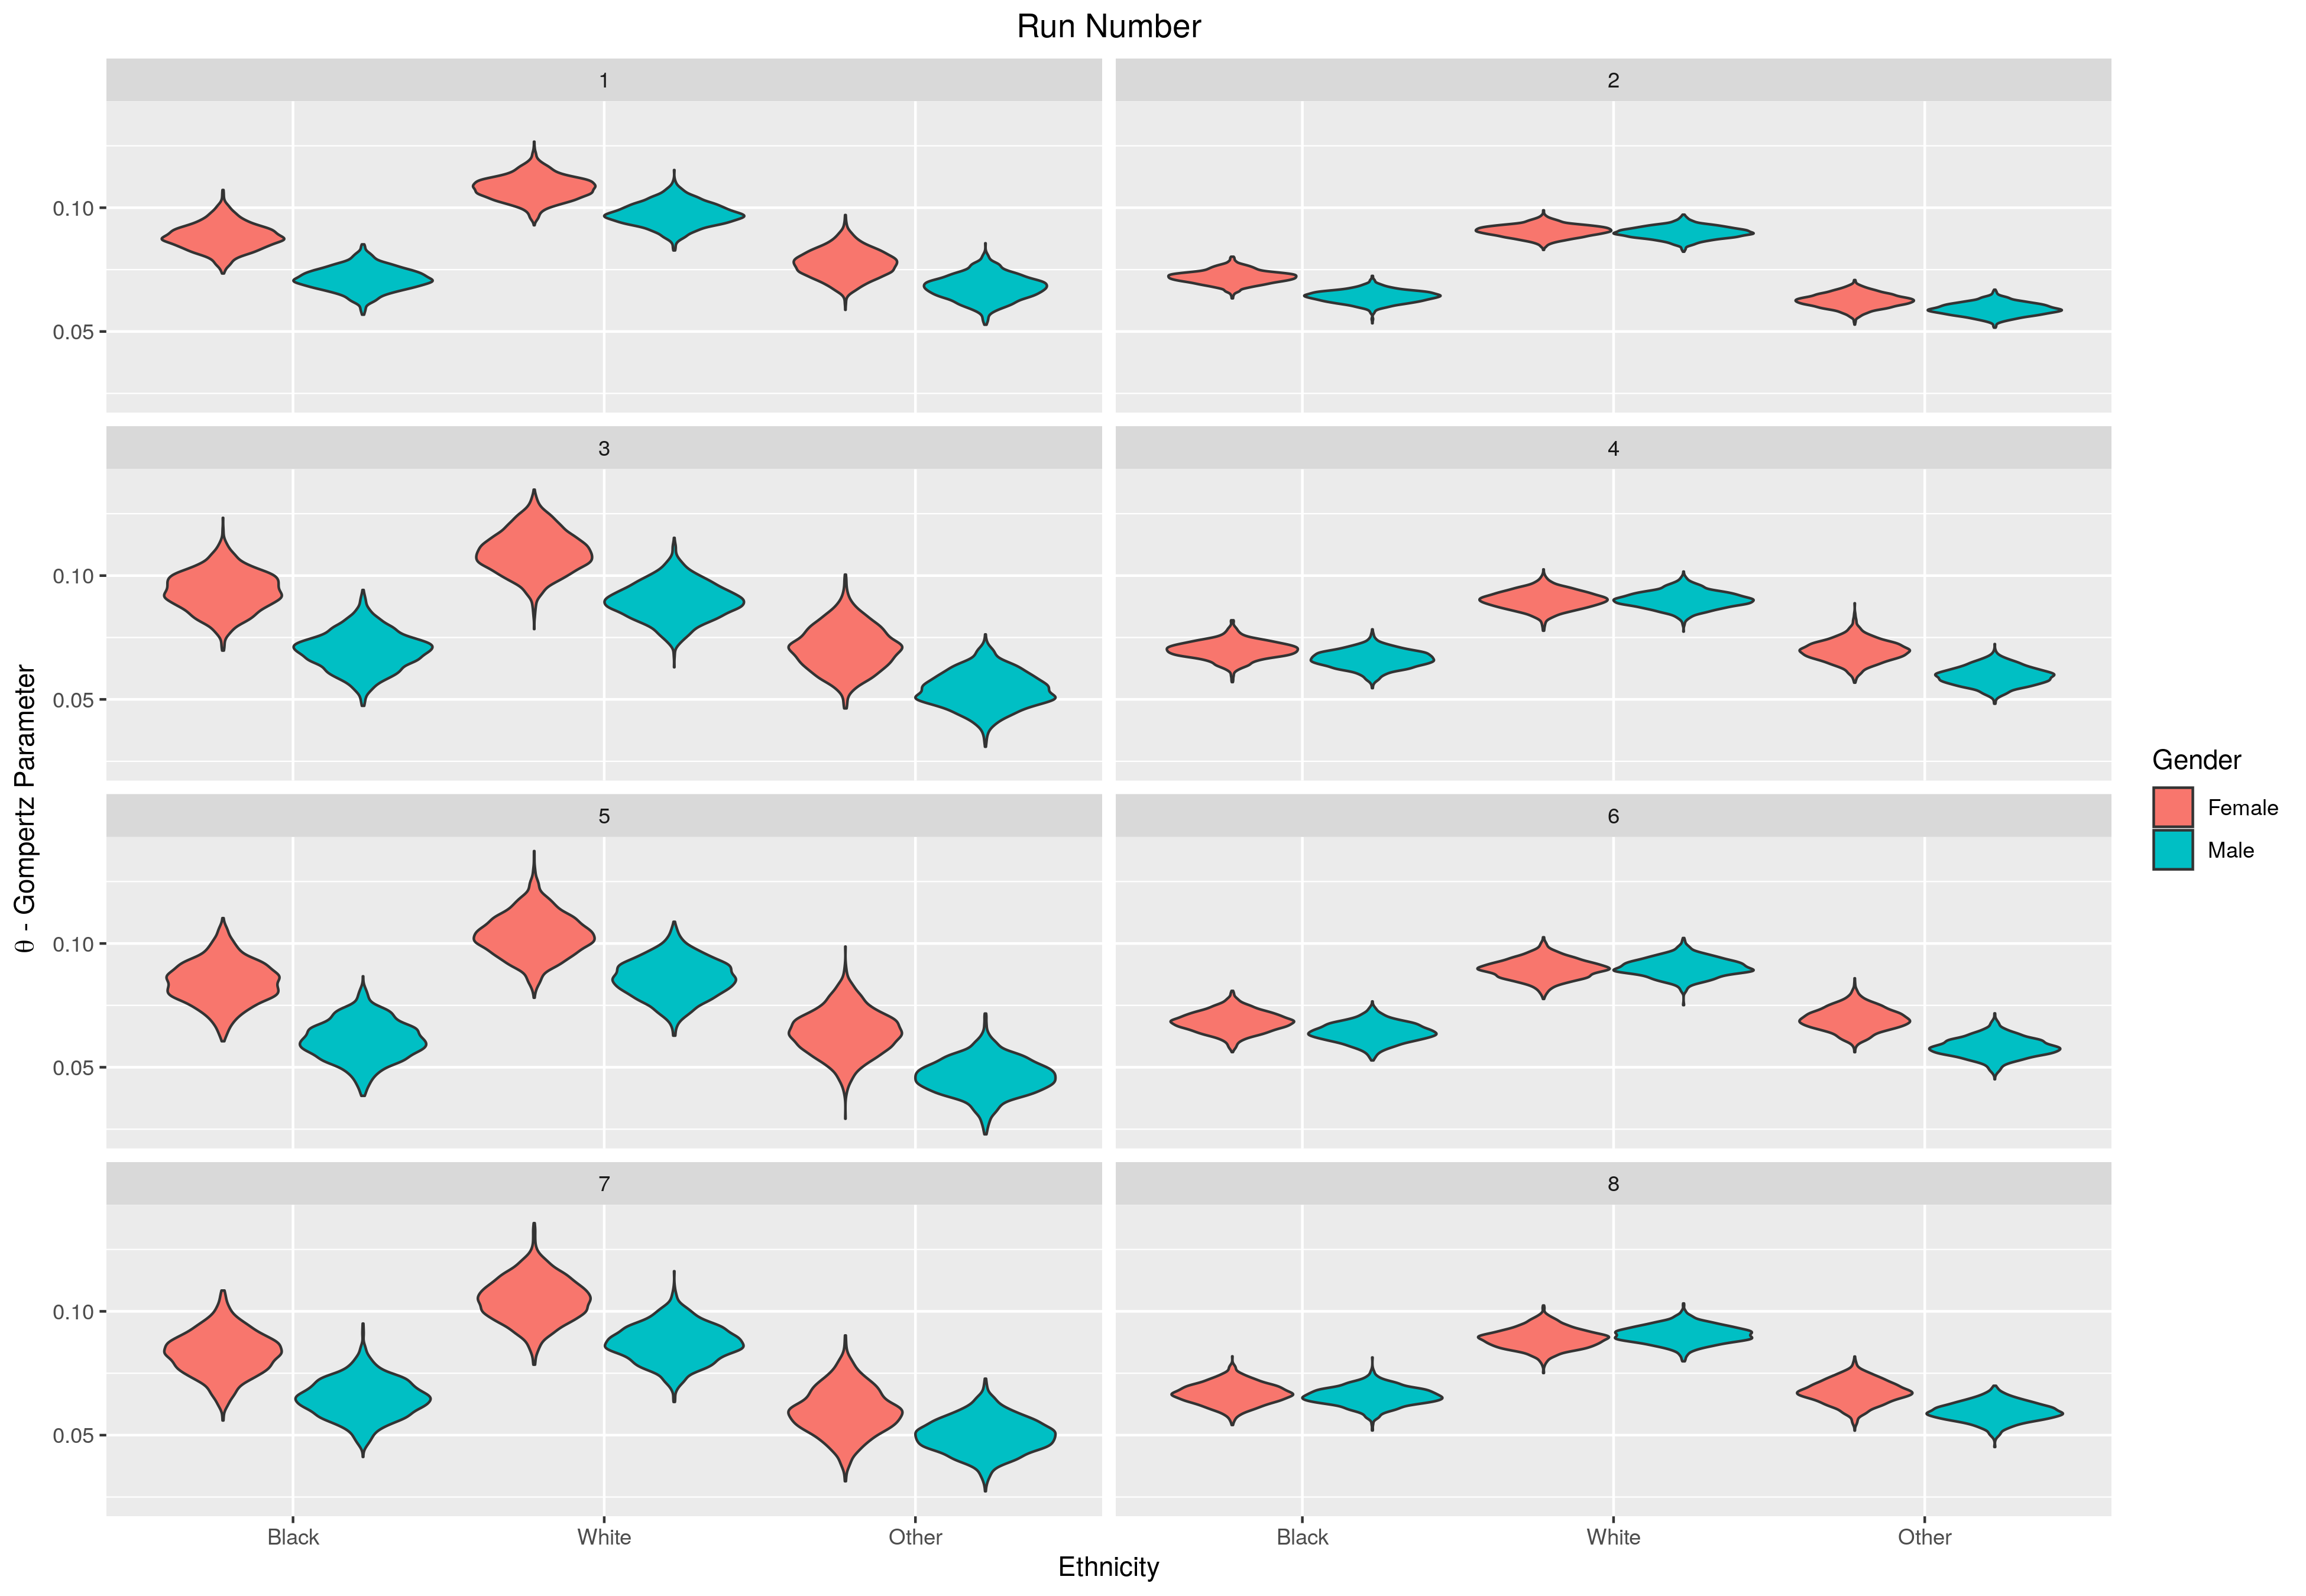
\includegraphics{./Plots/gompertz/theta_parameter.png}
\caption{Violin plots of the normalised \(\theta\) parameter (from the
Gompertz equation) of the different models.}\label{fig:gompt}
}
\end{figure}

To measure the performance of the model to predict the survival outcome
of individuals in the population, figure \ref{fig:cumpred} shows,
ordered by individual age, the cumulative hazard \(H(t)\) predicted
against the cumulative number of deaths in the populations, for each
model explored in this research. Each model is shown to predict survival
outcomes reliably, across the entire age range of the population.

\begin{figure}
\hypertarget{fig:cumpred}{%
\centering
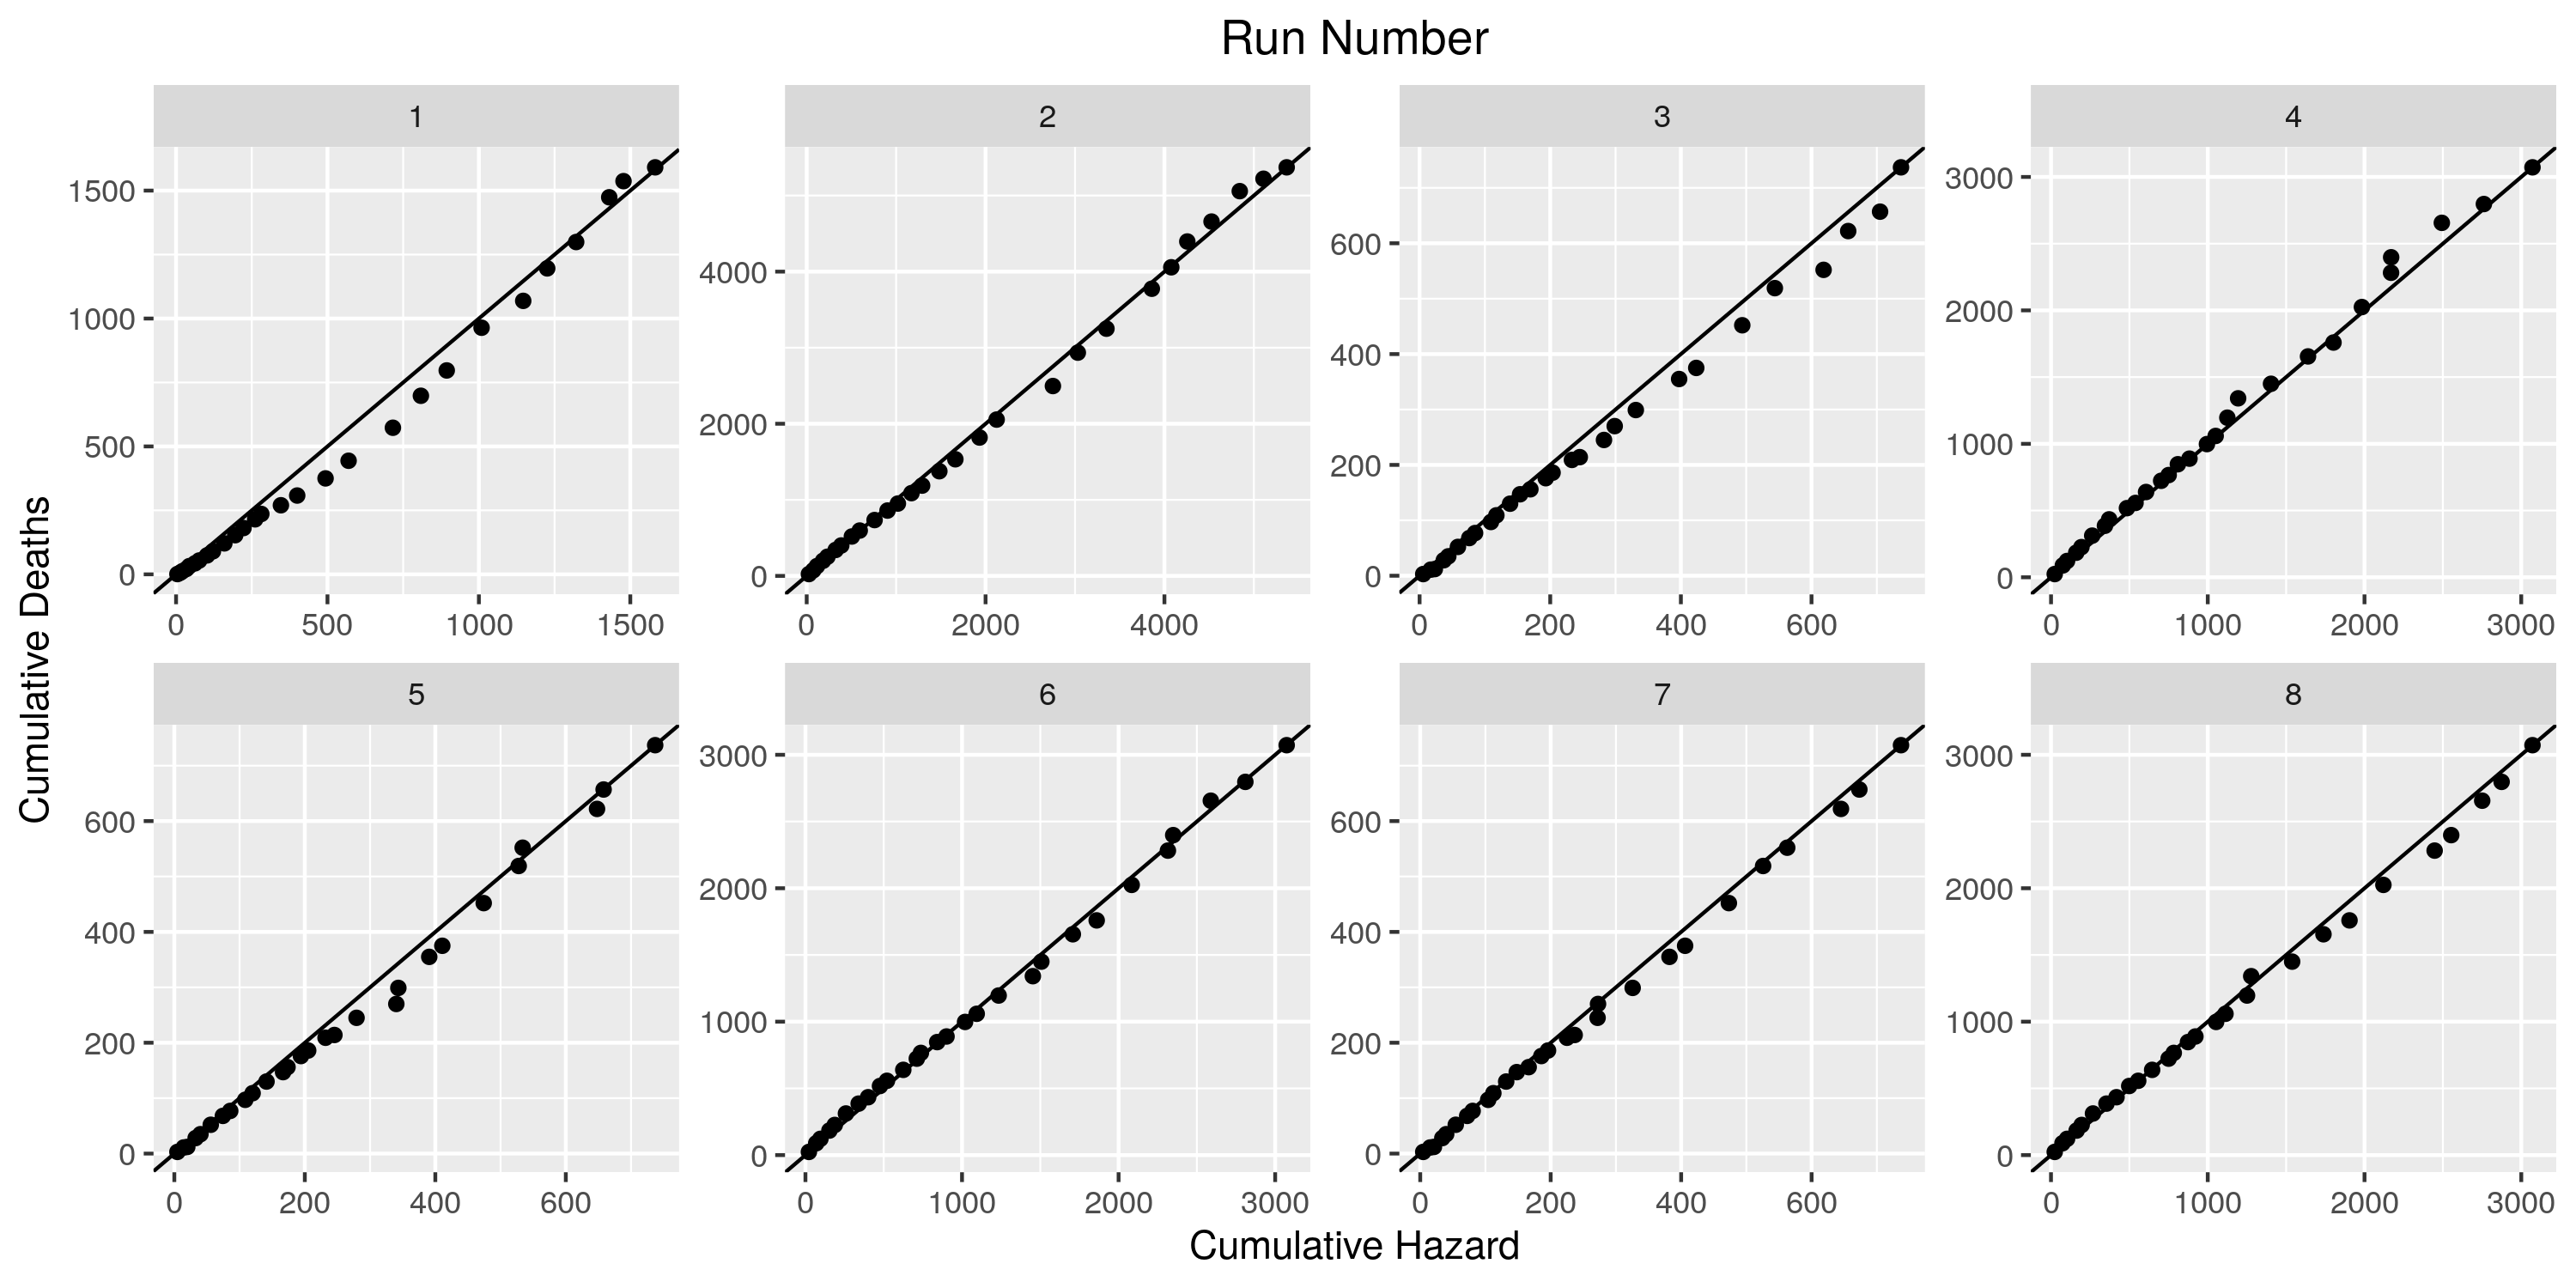
\includegraphics{./Plots/Survival/redlinpred_Cumulative_haz-death_age.png}
\caption{Predicted cumulative hazard against cumulative number of deaths
in the population, ordered by the age of the
individual.}\label{fig:cumpred}
}
\end{figure}

The concordance index is a method that can be used to evaluate the
accuracy of risk scores to predict survival outcomes between many
individuals in a given population. The best advantage of the concordance
index is for survey or census data that includes censoring. To see the
exact method for the concordance index presented below, including the
confidence intervals, please see M. J. Pencina and R.B D'Agostino
(2004). The concordance index compares all individuals that had a death
outcome with all other individuals that either died or was censored at a
later age than the first individual. For each couple, the risk scores
(in this work, this is the relative risk, \(h\)) are compared, and the
accuracy of the model is thereby reflected by having individuals with
lower risk scores outliving the other individual. For two individuals,
\(a\) and \(b\), whereby individual \(a\) had a death at time \(T_a\)
and individual \(b\) had either a death or was censored at time \(T_b\),
they are both said to be concordant if \(h_a>h_b\) and \(T_a<T_b\), and
discordant if \(h_a<h_b\) and \(T_a<T_b\). By evaluating this over the
entire population, this provides an estimation of the accuracy of using
the risk score to predict survival outcomes in the population. Table
@ref(tab:concord\_var) provides the concordance indices and their
\(\alpha=0.05\) confidence intervals for each of the different runs
(that correspond to table @ref(tab:runnumers)), for a variety of
different models.

\begin{tabular}{llllllllll}
\toprule
NA. & Model & Run.Number.1 & Run.Number.2 & Run.Number.3 & Run.Number.4 & Run.Number.5 & Run.Number.6 & Run.Number.7 & Run.Number.8\\
\midrule
1 & Full model & 0.564 (0.517-0.61) & 0.51 (0.487-0.533) & 0.624 (0.567-0.678) & 0.555 (0.528-0.582) & 0.555 (0.498-0.611) & 0.528 (0.501-0.555) & 0.578 (0.521-0.634) & 0.535 (0.508-0.562)\\
2 & FRS or mean systolic BP & 0.57 (0.523-0.615) & 0.516 (0.492-0.539) & 0.618 (0.561-0.672) & 0.551 (0.524-0.578) & 0.522 (0.464-0.578) & 0.513 (0.486-0.54) & 0.545 (0.487-0.601) & 0.521 (0.494-0.548)\\
3 & FRS or mean systolic & diastolic BP & 0.552 (0.505-0.597) & 0.505 (0.482-0.529) & 0.618 (0.561-0.672) & 0.551 (0.524-0.578) & 0.522 (0.464-0.578) & 0.513 (0.486-0.54) & 0.545 (0.487-0.601) & 0.521 (0.494-0.548)\\
4 & No short-term variation (sigmas) & 0.558 (0.511-0.603) & 0.507 (0.484-0.53) & 0.618 (0.561-0.672) & 0.55 (0.522-0.576) & 0.543 (0.486-0.6) & 0.523 (0.496-0.55) & 0.567 (0.51-0.623) & 0.53 (0.503-0.557)\\
5 & Gompertz only & 0.553 (0.507-0.599) & 0.54 (0.516-0.563) & 0.59 (0.532-0.644) & 0.558 (0.531-0.585) & 0.607 (0.55-0.662) & 0.564 (0.537-0.591) & 0.601 (0.543-0.655) & 0.563 (0.535-0.589)\\
\addlinespace
6 & No time or age dependency & 0.627 (0.581-0.671) & 0.599 (0.576-0.621) & 0.642 (0.585-0.695) & 0.59 (0.563-0.617) & 0.624 (0.567-0.678) & 0.58 (0.553-0.606) & 0.627 (0.57-0.68) & 0.58 (0.553-0.607)\\
\bottomrule
\end{tabular}

The results show that models that do not include time-at-outcome
information (by setting the Gompertz parameter, \(\theta\), to zero),
but still include blood pressure covariates are stronger predictors of
mortality risk, as compared to the full model. We find, as expected,
that models trained specifically on CVD and heart-attack related
mortality to be more accurate than trained on all mortality events.
Additionally, there does not appear to be a statistically significant
advantage of using either of the FRS covariates instead of the mean
systolic and diastolic blood pressure to predict survival outcomes. By
calculating the concordance index for specific demographic groups, we
can also evaluate the performance of the full models per group, as shown
in table @ref(tab:concord\_demo). The results indicate that the
performance of the predictions do vary between demographic groups. For
CVD and heart-attack mortality, the average concordance index for the
black female population was 0.58, black male population 0.52, other
female population 0.53, other male population 0.47, white female
population 0.55 and white male population 0.57. Therefore, the accuracy
of this model is visibly less accurate for the non-black or white ethnic
populations in the survey. On average across CVD and heart attack
mortality, the models were more accurate for the female population
(0.56) than the male population (0.53).

\begin{tabular}{llllllllll}
\toprule
NA. & Model & Run.Number.1 & Run.Number.2 & Run.Number.3 & Run.Number.4 & Run.Number.5 & Run.Number.6 & Run.Number.7 & Run.Number.8\\
\midrule
1 & Black & female & 0.568 (0.423-0.703) & 0.492 (0.425-0.56) & 0.659 (0.492-0.794) & 0.546 (0.473-0.616) & 0.555 (0.392-0.707) & 0.502 (0.43-0.574) & 0.586 (0.421-0.734) & 0.499 (0.428-0.571)\\
2 & Black & male & 0.542 (0.422-0.657) & 0.476 (0.417-0.535) & 0.572 (0.434-0.7) & 0.521 (0.457-0.585) & 0.48 (0.348-0.616) & 0.459 (0.395-0.523) & 0.507 (0.372-0.641) & 0.472 (0.408-0.536)\\
3 & Other & female & 0.532 (0.366-0.691) & 0.467 (0.392-0.542) & 0.549 (0.389-0.699) & 0.489 (0.41-0.569) & 0.545 (0.385-0.696) & 0.482 (0.403-0.562) & 0.525 (0.367-0.679) & 0.468 (0.389-0.548)\\
4 & Other & male & 0.533 (0.409-0.653) & 0.481 (0.421-0.542) & 0.548 (0.421-0.668) & 0.511 (0.443-0.579) & 0.395 (0.28-0.523) & 0.434 (0.368-0.503) & 0.425 (0.307-0.553) & 0.452 (0.385-0.52)\\
5 & White & female & 0.543 (0.45-0.632) & 0.45 (0.404-0.498) & 0.591 (0.45-0.719) & 0.494 (0.433-0.555) & 0.535 (0.396-0.669) & 0.468 (0.408-0.53) & 0.553 (0.413-0.685) & 0.477 (0.417-0.539)\\
\addlinespace
6 & White & male & 0.539 (0.459-0.617) & 0.465 (0.422-0.508) & 0.6 (0.477-0.712) & 0.504 (0.447-0.562) & 0.584 (0.461-0.697) & 0.479 (0.422-0.537) & 0.59 (0.467-0.702) & 0.485 (0.428-0.543)\\
\bottomrule
\end{tabular}

The concordance index can also be calculated using specific age-groups
of the population in order to evaluate the performance of the model for
each group. This can be shown to be equivalent to calculating the Area
Under the ROC Curve (AUC or AUROC) for each specific group. The results,
per run number, are illustrated in figure \ref{fig:timConc}. The plot
reflects that the expected value of the concordance index is highest
towards the bulk of the population - between roughly 50 to 80 years old,
with the performance either decreasing or with increasing confidence
intervals before and after this range.

\begin{figure}
\hypertarget{fig:timConc}{%
\centering
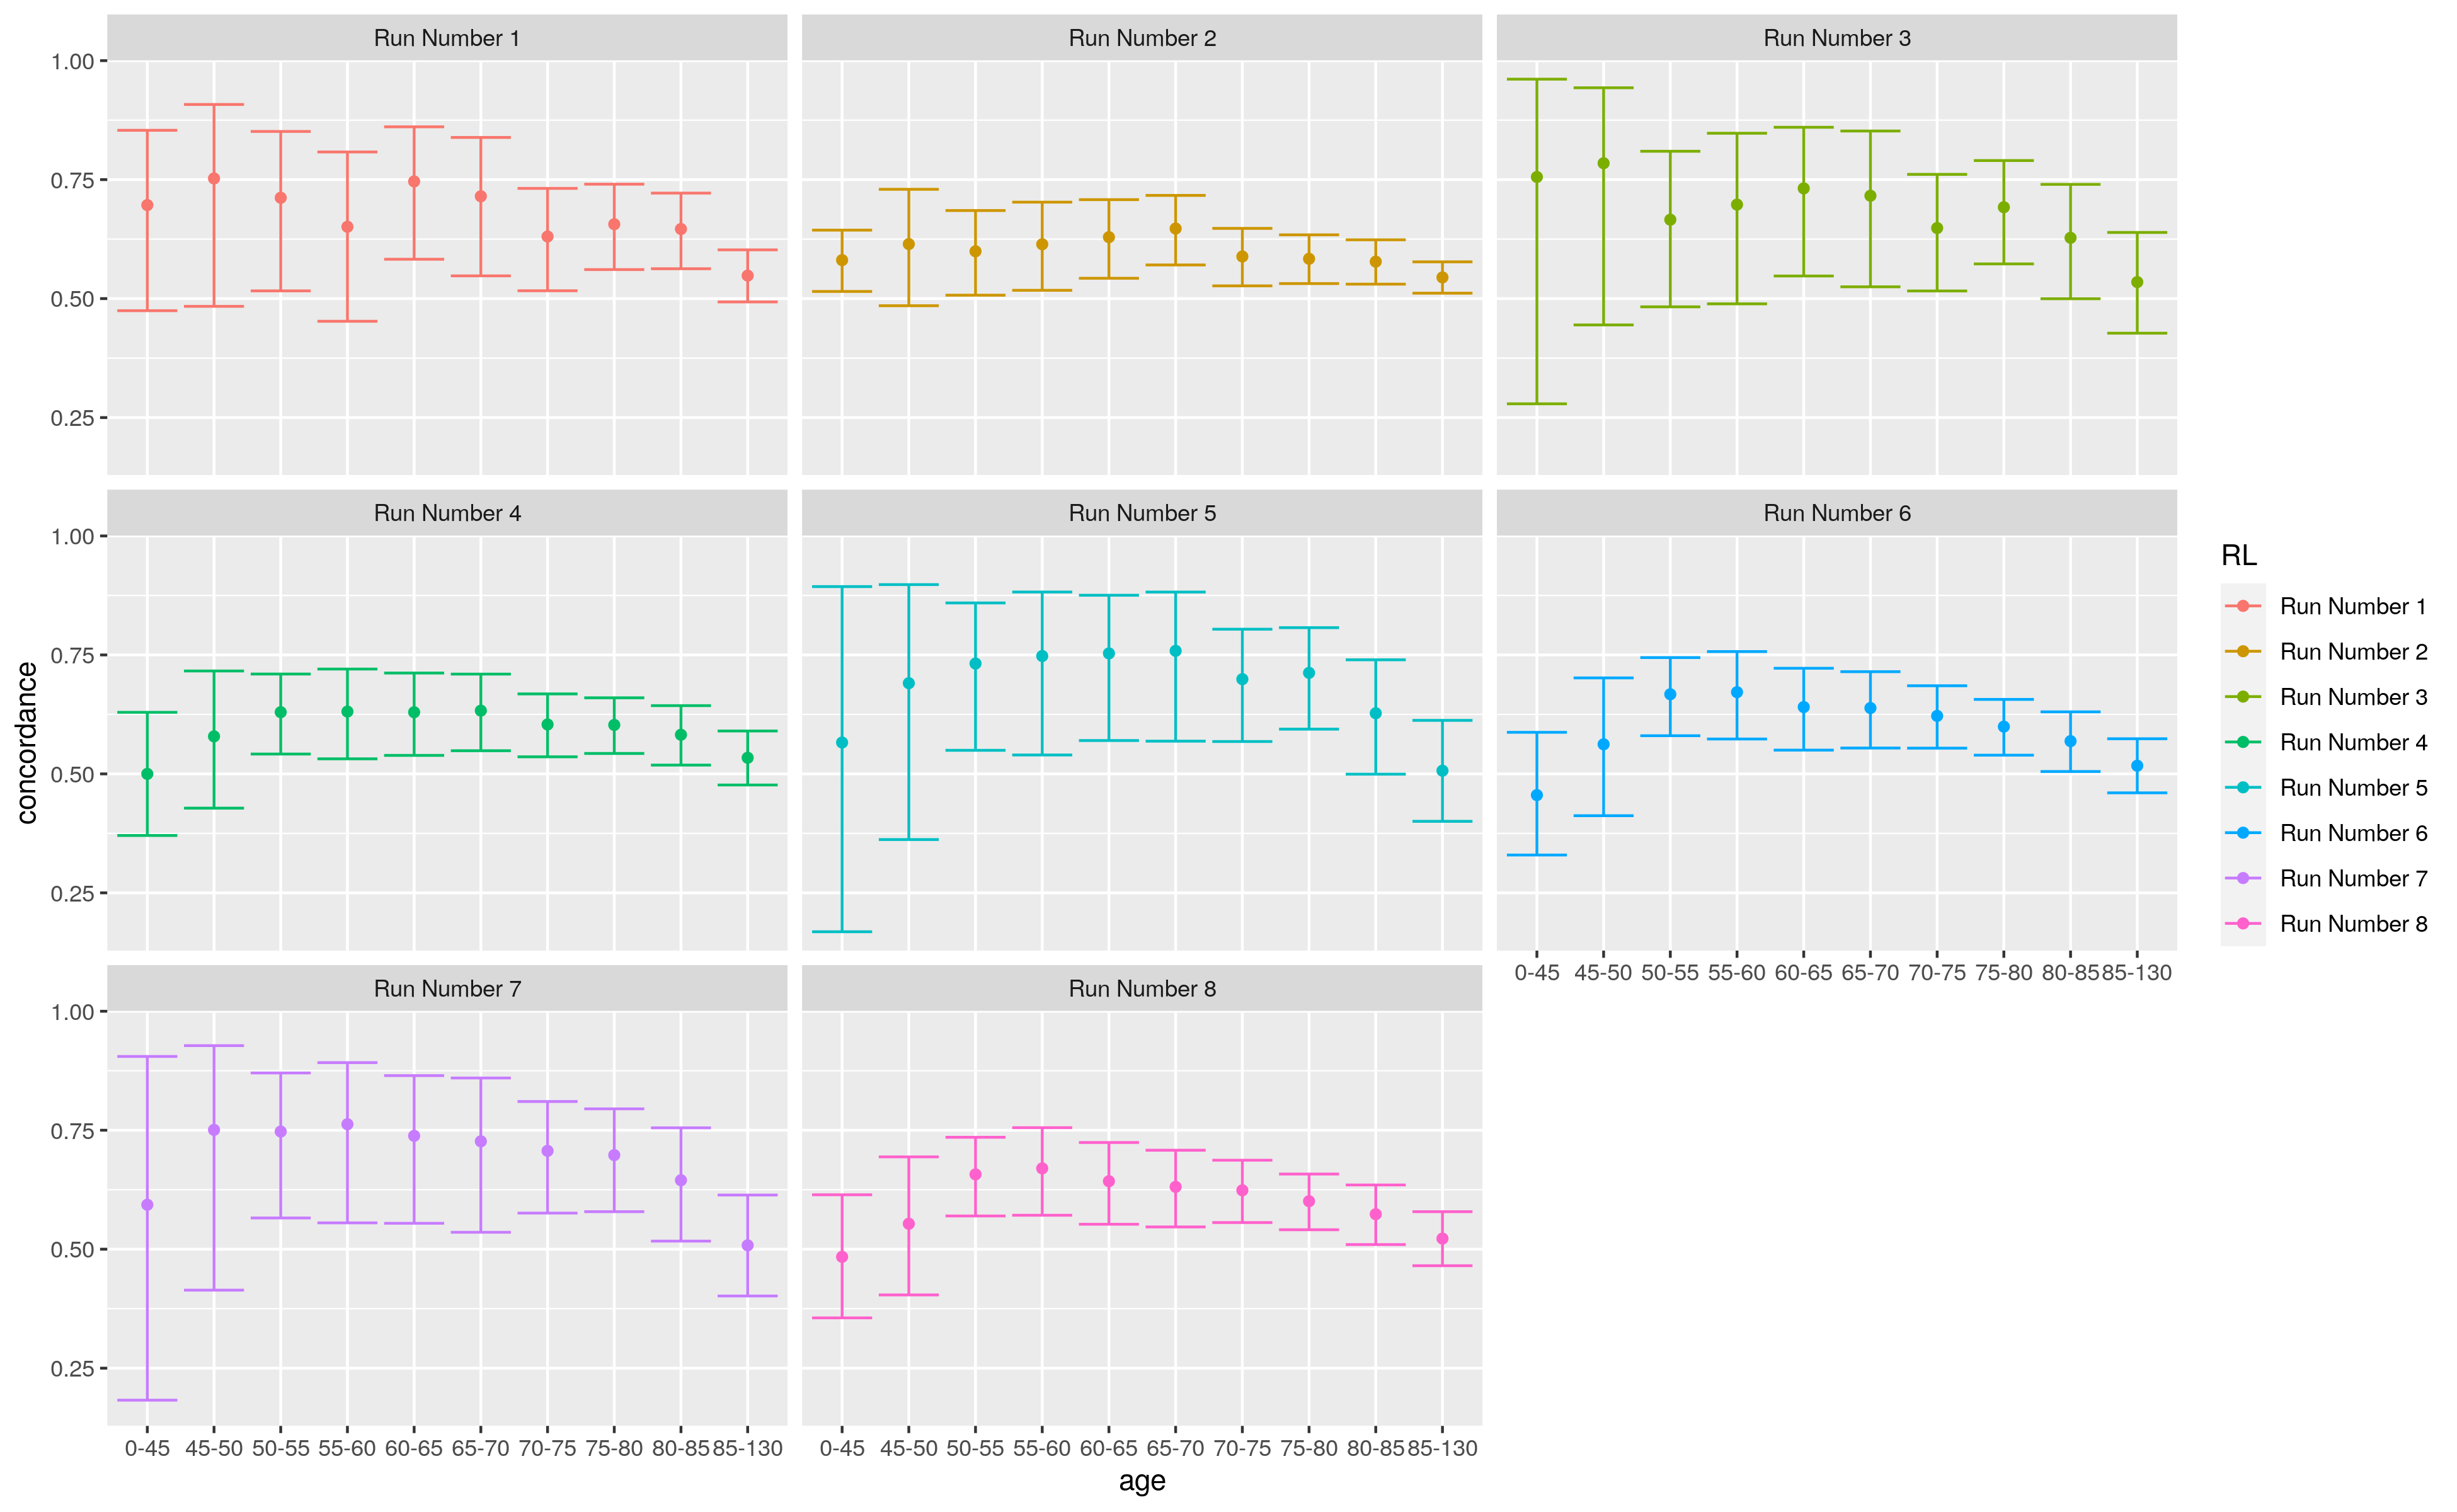
\includegraphics{./Plots/Survival/TimeDep_Concordance.png}
\caption{Time-dependent concordance index (AUC), per run
number.}\label{fig:timConc}
}
\end{figure}

\end{document}
